\documentclass[11pt]{article}

\usepackage[a4paper]{geometry}
\geometry{left=2.0cm,right=2.0cm,top=2.5cm,bottom=2.5cm}

% Chinese support
\usepackage{ctex}

% Math packages
\usepackage{amsmath,amsfonts,amssymb,amsthm,bm,mathrsfs,mathtools,breqn}

% Graphics and Colors
\usepackage{graphicx}
\usepackage{xcolor}
\usepackage{tikz}
\usetikzlibrary{arrows.meta,positioning}
\usepackage{pgfplots}
\pgfplotsset{compat=1.18}
\usepackage{circuitikz}
\graphicspath{{fig/}}

% Units
\usepackage{siunitx}

% Algorithms
\usepackage{algorithm}
\usepackage[noend]{algpseudocode}

% Layout and formatting
\usepackage{fancyhdr}
\usepackage[framemethod=TikZ]{mdframed}
\usepackage{fontspec}
\usepackage{fontsize}
\usepackage{adjustbox}
\usepackage{float}
\usepackage{multicol}
\usepackage{multirow}
\usepackage{pdfpages}
\usepackage{wrapfig}
\usepackage{subcaption}
\usepackage[inline]{enumitem}

% Tables
\usepackage{booktabs}
\usepackage{bigstrut,rotating}

% Listings
\RequirePackage{listings}

% Hyperlinks
\usepackage{hyperref}
\hypersetup{colorlinks=true,linkcolor=blue}

% Cross-referencing
\usepackage[capitalize]{cleveref}
\Crefname{section}{Section}{Sections}
\Crefname{table}{Table}{Tables}
\crefname{table}{Table.}{Tabs.}

% Listing settings
\definecolor{dkgreen}{rgb}{0,0.6,0}
\definecolor{gray}{rgb}{0.5,0.5,0.5}
\definecolor{mauve}{rgb}{0.58,0,0.82}

\lstset{
  frame=tb,
  aboveskip=3mm,
  belowskip=3mm,
  showstringspaces=false,
  columns=flexible,
  framerule=1pt,
  rulecolor=\color{gray!35},
  backgroundcolor=\color{gray!5},
  basicstyle={\small\ttfamily},
  numbers=none,
  numberstyle=\tiny\color{gray},
  keywordstyle=\color{blue},
  commentstyle=\color{dkgreen},
  stringstyle=\color{mauve},
  breaklines=true,
  breakatwhitespace=true,
  tabsize=3,
}

\setmainfont{Palatino Linotype}
\setCJKmainfont{SimSun}[BoldFont=SimHei, ItalicFont=KaiTi]
\setCJKsansfont{SimHei}
\setCJKmonofont{FangSong}
\punctstyle{kaiming}
% 偏好的几个字体, 可以根据需要自行加入字体ttf文件并调用

% Restore standard emphasis to avoid requiring an undefined environment (kaishu).
% The original redefinition used an environment `kaishu` which is not defined
% in a default ctex setup and causes compilation errors. Use \textit for
% emphasis which works across engines.
\renewcommand{\emph}[1]{\textit{#1}}

%改这里可以修改实验报告表头的信息
\newcommand{\experiName}{磁滞回线}
\newcommand{\supervisor}{朱中柱}
\newcommand{\name}{邓思豪}
\newcommand{\studentNum}{2023K8009909008}
\newcommand{\class}{3}
\newcommand{\group}{01}
\newcommand{\seat}{5}
\newcommand{\dateYear}{2025}
\newcommand{\dateMonth}{12}
\newcommand{\dateDay}{31}
\newcommand{\room}{学二340}
\newcommand{\others}{$\square$}


\begin{document}



\begin{center}
    \LARGE \bf 《\, 基\, 础\, 物\, 理\, 实\, 验\, 》\, 实\, 验\, 报\, 告
\end{center}

\begin{center}
    \noindent \emph{实验名称}\underline{\makebox[25em][c]{\experiName}}
    \emph{指导教师}\underline{\makebox[8em][c]{\supervisor}}\\
    \emph{姓名}\underline{\makebox[6em][c]{\name}} 
    % 如果名字比较长, 可以修改box的长度"6em"
    \emph{学号}\underline{\makebox[10em][c]{\studentNum}}
    \emph{分班分组及座号} \underline{\makebox[5em][c]{\class \ -\ \group \ -\ \seat }\emph{号}} （\emph{例}:\, 1\,-\,04\,-\,5\emph{号}）\\
    \emph{实验日期} \underline{\makebox[3em][c]{\dateYear}}\emph{年}
    \underline{\makebox[2em][c]{\dateMonth}}\emph{月}
    \underline{\makebox[2em][c]{\dateDay}}\emph{日}
    \emph{实验地点}\underline{{\makebox[6em][c]\room}}
    \emph{调课/补课} \underline{\makebox[3em][c]{\others\ 是}}
    \emph{成绩评定} \underline{\hspace{5em}}
    {\noindent}
    \rule[8pt]{17cm}{0.2em}
\end{center}

\section{实验目的}

\begin{enumerate}
    \item 掌握利用示波器测量铁磁材料动态磁滞回线的方法；
    \item 掌握利用霍尔传感器测量铁磁材料（准）静态磁滞回线的方法；
    \item 了解铁磁性材料的磁化特性；
    \item 了解磁滞、磁滞回线和磁化曲线的概念，加深对饱和磁化强度、剩余磁化强度、矫顽力等物理量的理解。
\end{enumerate}

\section{实验仪器与用具}

\begin{enumerate}
    \item 磁特性综合测量实验仪（包括正弦波信号源，待测样品及绕组，积分电路所用的电阻和电容）。双踪示波器，直流电源，电感，数字多用表。
    
    磁特性综合测量实验仪主要技术指标如下：
    \begin{enumerate}[label=\arabic*)]
        \item 样品 1：锰锌铁氧体，圆形罗兰环，磁滞损耗较小。平均磁路长度 $l=\SI{0.130}{\meter}$，铁芯实验样品截面积 $S=\SI{1.24e-4}{\meter\squared}$，线圈匝数：$N_1=150$ 匝，$N_2=150$ 匝；$N_3=150$ 匝。
        \item 样品 2：EI 型硅钢片，磁滞损耗较大。平均磁路长度 $l=\SI{0.075}{\meter}$，铁芯实验样品截面积 $S=\SI{1.20e-4}{\meter\squared}$，线圈匝数：$N_1=150$ 匝，$N_2=150$ 匝；$N_3=150$ 匝。
        \item 信号源的频率在 \SIrange{20}{200}{\hertz} 间可调；可调标准电阻 $R_1$、$R_2$ 均为无感交流电阻，$R_1$ 的调节范围为 \SIrange{0.1}{11}{\ohm}；$R_2$ 的调节范围为 \SIrange{1}{110}{\kilo\ohm}。标准电容有 \SIrange{0.1}{11}{\micro\farad} 可选。
    \end{enumerate}

    \item 磁性材料磁滞回线和磁化曲线测定仪（包括数字式特斯拉计、恒流源、磁性材料样品、磁化线圈、双刀双掷开关、霍耳探头移动架、双叉头连接线、箱式实验平台）。
    
    其主要技术指标如下：
    \begin{enumerate}[label=\arabic*)]
        \item 数字式特斯拉计：四位半 LED 显示，量程 \SI{2.000}{\tesla}；分辨率 \SI{0.1}{\milli\tesla}；带霍耳探头。
        \item 恒流源：四位半 LED 显示，可调恒定电流 \SIrange{0}{600.0}{\milli\ampere}。
        \item 磁性材料样品：条状矩形结构，截面长 \SI{2.00}{\centi\meter}；宽 \SI{2.00}{\centi\meter}；隔隙 \SI{2.00}{\milli\meter}；平均磁路长度 $\bar{l}=\SI{0.240}{\meter}$（样品与固定螺丝为同种材料）。
        \item 磁化线圈总匝数 $N=2000$。
    \end{enumerate}
\end{enumerate}

\section{实验原理}
\label{sec:principles}

\subsection{铁磁材料的磁化特性}
\label{subsec:mag_properties}

把物体放在外磁场 $H$ 中，物体就会被磁化。其内部产生磁场。设其内部磁化强度为 $M$，磁感应强度为 $B$，可以定义磁化率 $\chi_m$ 和相对磁导率 $\mu_r$ 表示物质被磁化的难易程度：
\begin{equation}
    \chi_m = \frac{M}{H}
\end{equation}
\begin{equation}
    \mu_r = \frac{B}{\mu_0 H}
\end{equation}
其中，$\mu_0$ 是真空磁导率（$\mu_0 = 4\pi \times 10^{-7} \text{ N/A}^2$）。由于 $B = \mu_0(M + H)$，因此 $\mu_r = 1 + \chi_m$。

物质的磁性按磁化率可以分为抗磁性、顺磁性和铁磁性三种。抗磁性物质的磁化率为负值，通常在 $10^{-5} \sim 10^{-6}$ 的量级，且几乎不随温度变化；顺磁性物质的磁化率通常为 $10^{-2} \sim 10^{-4}$ 之间，且随温度线性增大；而铁磁性物质的磁化率通常大于 1，且随温度增高而变小。铁磁性材料主要是铁、钴、镍及它们的合金和氧化物，以及稀土与过渡族元素组成的合金等。由于铁磁材料的磁导率很高，常被用作电感、电磁铁、变压器的铁芯材料，以增大线圈中的磁通量。

除了磁导率高以外，铁磁材料还具有特殊的磁化规律。对于一个处于磁中性状态（$H=0, B=0$）的铁磁材料加上由小变大的磁场 $H$ 进行磁化时，$B$ 随 $H$ 的变化曲线称为起始磁化曲线，它大致分为三个阶段：
(1) 可逆磁化阶段（图\ref{fig:hysteresis_loop}中的 OA 段）；
(2) 不可逆磁化阶段（见图\ref{fig:hysteresis_loop}中 AS 段）；
(3) 饱和磁化阶段（见图\ref{fig:hysteresis_loop}中 SC 段）。

在 S 点材料已经被磁化至饱和状态，继续增大 $H$，磁化强度 $M$ 不再增大，由于 $B = \mu_0(M + H)$，$B$ 会随 $H$ 线形增大，但增量极小。图中 $H_s$ 和 $B_s$ 表示 $M$ 刚刚达到饱和值时的 $H$ 和 $B$ 的值，分别称为饱和磁场强度和饱和磁感应强度。

如果将铁磁材料磁化到饱和状态后再减小磁场 $H$，那么磁感应强度 $B$ 会随 $H$ 减小而减小，但并不沿起始磁化曲线 SAO 减小，而是沿着 SP 这条更缓慢的曲线减小。当 $H$ 减小到 0 时，$B$ 并不为 0，$H$ 称为矫顽力 $H_c$。

% 插入图片 1 & 2 对应的示意图
% [此处应插入图片：图 1 铁磁材料的起始磁化曲线和饱和磁滞回线示意图]
\begin{figure}[H]
    \centering
    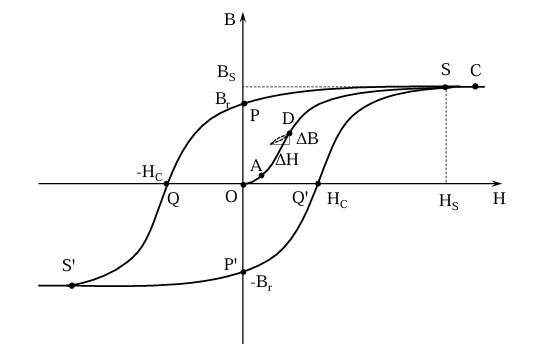
\includegraphics[width=0.6\textwidth]{figure1.png}
    \caption{铁磁材料的起始磁化曲线和饱和磁滞回线示意图}
    \label{fig:hysteresis_loop}
\end{figure}

如果磁场在任意 $[-H_m, H_m]$ 范围内作循环变化，那么 $B$ 也会做循环变化，形成一个闭合的磁滞回线。磁滞回线的面积对应于循环磁化一周所发生的能量损耗。


\begin{figure}[H]
    \centering
    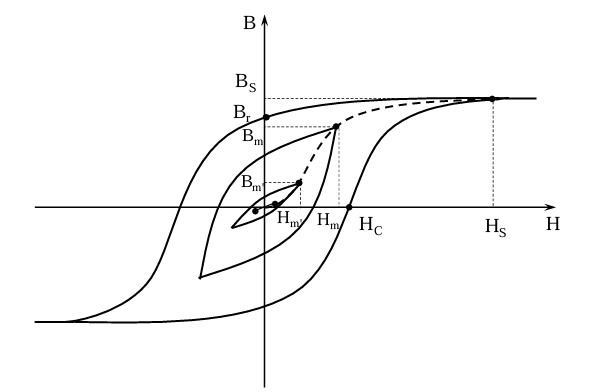
\includegraphics[width=0.6\textwidth]{figure2.png}
    \caption{铁磁材料的动态磁滞回线和动态磁化曲线示意图}
    \label{fig:dynamic_loop}
\end{figure}

动态磁滞回线形状与磁化场频率和幅度都有关。在同一频率下，交变磁场幅度不同时，动态磁滞回线也会不同。将磁场幅值从 0 增到 $H_s$，这些动态磁滞回线的顶点 $(H_m, B_m)$ 的连线称为动态磁化曲线（见图\ref{fig:dynamic_loop}）。在这条曲线上任意一点的 $B_m$ 和对应 $H_m$ 的比值 $\mu_m = \frac{B_m}{\mu_0 H_m}$ 称为振幅磁导率。

对于起始磁化曲线起始的可逆阶段，可以定义起始磁导率为：
\begin{equation}
    \mu_i = \lim_{H \to 0} \frac{B}{\mu_0 H}
\end{equation}

在有直流偏置又叠加弱交变磁场的情况下，相关的磁导率称为可逆磁导率 $\mu_R$：
\begin{equation}
    \mu_R = \lim_{\Delta H \to 0} \frac{\Delta B}{\mu_0 \Delta H}
\end{equation}

\subsection{动态磁滞回线的测量}
\label{subsec:dynamic_measure}

测量动态磁滞回线的原理电路如图\ref{fig:circuit_dynamic}所示。


% [此处应插入图片：图 3 用示波器测量动态磁滞回线电路图]
\begin{figure}[H]
    \centering
    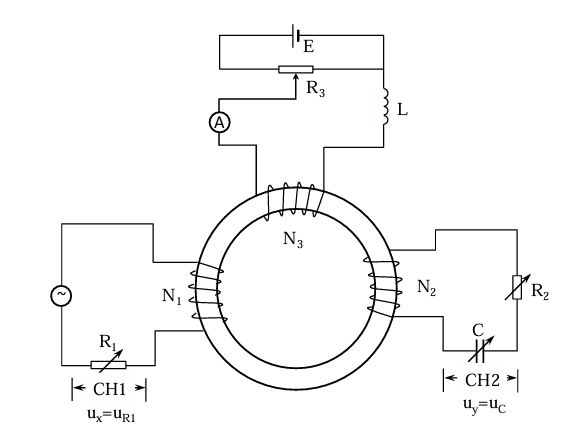
\includegraphics[width=0.7\textwidth]{figure3.png}
    \caption{用示波器测量动态磁滞回线电路图}
    \label{fig:circuit_dynamic}
\end{figure}

交流磁场强度 $H$ 的测量原理。正比于励磁电流 $i_1$：
\begin{equation}
    H = \frac{N_1}{l} i_1
\end{equation}
由于 $i_1 = u_{R_1}/R_1$，因此：
\begin{equation}
    H = \frac{N_1}{l R_1} u_{R_1} \quad 
\end{equation}

交流磁感应强度 $B$ 的测量原理。线圈 2 上的感应电压 $u_2$ 为：
\begin{equation}
    u_2 = -\frac{N_2 d\Phi}{dt} = -\frac{N_2 S dB}{dt}
\end{equation}
通过 RC 积分电路后，电容 $C$ 上的电压 $u_C$ 为：
\begin{equation}
    u_C = \frac{Q}{C} = \frac{1}{C} \int i_2 dt \approx \frac{1}{CR_2} \int u_2 dt
\end{equation}
最终得出：
\begin{equation}
    B = \frac{R_2 C}{N_2 S} u_C \quad 
\end{equation}

\subsection{(准)静态磁化曲线和磁滞回线的测量}
\label{subsec:static_measure}

如果对绕上磁化线圈的铁磁材料样品施加直流激励，便会在样品中产生稳定的磁场。


% [此处应插入图片：图 4 （左）磁化曲线和磁滞回线，（右）基本磁化曲线]
\begin{figure}[H]
    \centering
    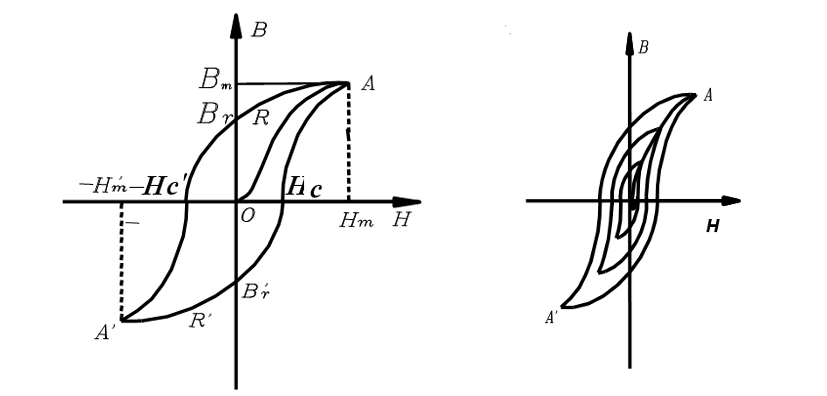
\includegraphics[width=0.7\textwidth]{figure4.png}
    \caption{(左) 磁化曲线和磁滞回线，(右) 基本磁化曲线}
    \label{fig:static_curves}
\end{figure}

用霍尔传感器测量（准）静态磁滞回线的原理电路如图\ref{fig:circuit_static}所示。

% [此处应插入图片：图 5 磁滞回线和磁化曲线测量装置]
\begin{figure}[H]
    \centering
    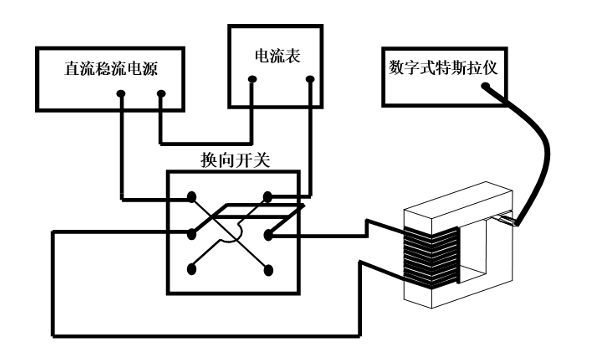
\includegraphics[width=0.6\textwidth]{figure5.png}
    \caption{磁滞回线和磁化曲线测量装置}
    \label{fig:circuit_static}
\end{figure}

磁场强度 $H$ 计算公式：
\begin{equation}
    H = \frac{N}{\bar{l}} I \quad 
\end{equation}
在实际测量中，由于缝隙 $\ell_g$ 的存在，需由安培环路定律进行修正：
\begin{equation}
    H \bar{l} + H_g \ell_g = NI \quad 
\end{equation}
由于磁通连续性 $B_g S_g = BS$，在缝隙很窄的情况下 $S_g \approx S$，则 $B \approx B_g$。
在空气隙中 $\mu_r = 1$，故 $H_g = B / \mu_0$。代入得：
\begin{equation}
    H \bar{l} + \frac{1}{\mu_0} B \ell_g = NI \quad 
\end{equation}
若 $\frac{1}{\mu_0} B \ell_g$ 对 $H \bar{l}$ 不可忽略时，可利用上式对 $H$ 值进行修正。

\section{实验内容}

\subsection{第一部分 用示波器观测动态磁滞回线}

\subsubsection{1. 观测样品 1（铁氧体）的饱和动态磁滞回线}

\begin{enumerate}
    \item 测量频率 $f=100\text{ Hz}$ 时的饱和磁滞回线。取 $R_1=2.0\ \Omega$, $R_2=50\text{ k}\Omega$, $C=10.0\ \mu\text{F}$。示波器选择 X-Y 模式。调节励磁电流大小及示波器的垂直、水平位移旋钮，在示波器显示屏上调出一个相对于坐标原点对称的饱和磁滞回线。测量并画出饱和磁滞回线的 $B-H$ 图。上下半支各选取 9 个以上的测量点。测量 $B_s, B_r, H_c$。可通过示波器光标（cursor）来读数。
    
    \item 保持信号源幅度不变，在仪器频率可调范围内，观测不同频率时的饱和磁滞回线。用不同频率时，磁滞回线有何变化？为什么？保持 $R_1, R_2C$ 不变，测量并比较 $f=95\text{ Hz}$ 和 $150\text{ Hz}$ 时的 $B_r$ 和 $H_c$。
    
    \item 在频率 $f=50\text{ Hz}$ 下，比较不同积分常数取值对李萨如图形的影响。固定励磁电流幅度 $I_m=0.1\text{ A}$, $R_1=2.0\ \Omega$，改变积分常数 $R_2C$。调节 $R_2C$ 分别为 $0.01\text{ s}, 0.05\text{ s}, 0.5\text{ s}$，观察并粗略画出不同积分常数下 $u_{R_1}-u_C$ 李萨如图形的示意图。请思考为什么积分常数会影响 $u_{R_1}-u_C$ 李萨如图形的形状？积分常数是否会影响真实的 $B-H$ 磁滞回线的形状？
\end{enumerate}

\subsubsection{2. 测量样品 1（铁氧体）的动态磁滞回线。（测量前需要对样品进行退磁。）}

\begin{enumerate}
    \item 在 $f=100\text{ Hz}$ 时，调出不同幅度的动态磁滞回线，测量并画出动态磁化曲线。取 $R_1=2.0\ \Omega, R_2=50\text{ k}\Omega, C=10.0\ \mu\text{F}$。磁场幅度 $H_m$ 从 0 到 $H_s$ 单调增加，要求至少 20 个测量点。
    \item 根据测量数据计算并画出 $\mu_m - H_m$ 曲线。
    \item 测定起始磁导率 $\mu_i$。
\end{enumerate}

\subsubsection{3. 观察不同频率下样品 2（硅钢）的动态磁滞回线}

取 $R_1=2.0\ \Omega, R_2=50\text{ k}\Omega, C=10.0\ \mu\text{F}$。在给定交变磁场幅度 $H_m=400\text{ A/m}$ 下，测量 $f=20\text{ Hz}, 40\text{ Hz}, 60\text{ Hz}$ 的 $B_m, B_r, H_c$。

\subsubsection{*4. 测量样品 1（铁氧体）在不同直流偏置磁场 $H$ 下的可逆磁导率。（测量前需要先对样品进行退磁。）}

交流磁场频率取 $f=100\text{ Hz}$。电路参数设置为：$R_1=2.0\ \Omega, R_2=20\text{ k}\Omega, C=2.0\ \mu\text{F}$。直流偏置磁场必须从 0 到 $H_s$ 单调增加。测量时，为保证精度，需调交流信号源幅度使交流磁场 $\Delta H$ 足够小，并调节示波器，使李萨如图充分放大，以观测磁化是否可逆。画出 $\mu_R - H$ 曲线（至少 10 个点）。

\subsection{第二部分 用霍尔传感器测量铁磁材料（准）静态磁滞回线}

\subsubsection{1. 测量模具钢样品的起始磁化曲线}

\begin{enumerate}
    \item[1)] 选择合适的电流与磁感应强度 $B$，用数字式特斯拉计测量样品间隙中剩磁的磁感应强度 $B$ 与位置 $X$ 的关系，$X$ 从 $-10\text{ mm}$ 到 $10\text{ mm}$，间隔 $1\text{ mm}$ 测一组数据，求得间隙中磁感应强度 $B$ 的均匀区范围 $\Delta X$ 值，将霍尔传感器放在测出的均匀区的中央。
    
    \item[2)] 对样品进行退磁处理。其方法是利用双刀开关使磁化电流不断反向，且幅值由最大值逐渐减小至零，最终使样品的剩磁 $B$ 为零。例如将电流值由 0 增至 $600\text{ mA}$ 再逐渐减小至 0，然后双刀开关换为反向电流由 0 增至 $500\text{ mA}$，再由 $500\text{ mA}$ 调至零，这样磁化电流不断反向，最大电流值每次减小 $100\text{ mA}$，当剩磁减小到 $100\text{ mT}$，每次最大电流减小量还需小些，最后将剩磁消除。然后测量 $B-H$ 关系曲线。至少获取 20 个采样点的实验数值。
\end{enumerate}

\subsubsection{2. 测量模具钢的磁滞回线}

\begin{enumerate}
    \item[1)] 测量模具钢的磁滞回线前的磁锻炼。由初始磁化曲线可以得到 $B$ 增加十分缓慢时，磁化线圈通过的电流值 $I_m$，然后保持此电流 $I_m$ 不变，把双刀换向开关来回拨动 8-10 次，进行磁锻炼。（开关拉动时，应使触点从接触到断开的时间长些，这是为什么？磁锻炼的作用是什么？）
    
    \item[2)] 测量模具钢的磁滞回线。通过磁化线圈的电流从饱和电流 $I_m$ 开始逐步减小到 0，然后双刀换向开关将电流换向，电流又从 0 增加到 $-I_m$，重复上述过程，即 $(H_m, B_m) \to (-H_m, -B_m)$，再从 $(-H_m, -B_m) \to (H_m, B_m)$。每隔 $50\text{ mA}$ 测一组 $(I_i, B_i)$ 值。
\end{enumerate}

\subsubsection{3. 数据处理及绘图}

由公式(3)求出 $H_i$ 值。测量模具钢样品的平均磁路长度 $\bar{l}$ 和间隙宽度 $\ell_g$，用公式(7)对 $H_i$ 进行修正。用作图纸作模具钢材料的起始磁化曲线和磁滞回线，记录模具钢的饱和磁感应强度 $B_m$、饱和磁场强度 $H_m$ 和矫顽力 $H_c$。

\vspace{1em}
\noindent \textbf{附：样品结构示意图}

\begin{figure}[H]
    \centering
    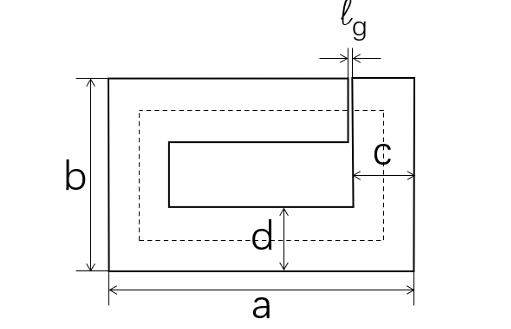
\includegraphics[width=0.5\textwidth]{sample_diagram.png}
    \caption{待测样品结构示意图}
    \label{fig:sample_diagram}
\end{figure}

$a=\SI{10.00}{\centi\meter}; b=\SI{6.00}{\centi\meter}; c=d=\SI{2.00}{\centi\meter}; \bar{l}$ 为样品平均长度（即样品中央轴线长度，如图中虚线所示）；$\ell_g$ 为平行间隙长度，$\ell_g=\SI{0.20}{\centi\meter}$。

\section{实验数据与分析}  
\subsection{用示波器观测动态磁滞回线}

\subsubsection{样品 1（铁氧体）的饱和动态磁滞回线}

(1) 测量绘制频率 $f=\SI{100}{\hertz}$ 时的饱和磁滞回线。取 $R_1=\SI{2.0}{\ohm}$，$R_2=\SI{50}{\kilo\ohm}$，$C=\SI{10.0}{\micro\farad}$。

\begin{table}[h!]
    \centering
    \caption{饱和磁滞回线（竖直方向成对测量）}
    \renewcommand{\arraystretch}{1.5} % 增加行高以容纳手写数据
    \begin{tabular}{ccc}
        \toprule
        (H) / (B) & 数据点 1 & 数据点 2 \\ 
        \midrule
        $H_S\ = \SI{90.4}{\milli\volt}$ & $B_S = \SI{21.2}{\milli\volt}$ &  \\
        $-H_S\ = \SI{-92.8}{\milli\volt}$ & $-B_S = \SI{-15.2}{\milli\volt}$ &  \\
        $0$ & $B_r = \SI{3.4}{\milli\volt}$ & $-B_r = \SI{-3.4}{\milli\volt}$ \\
        $-H_c = \SI{-7.20}{\milli\volt}$ & $0$ & $B_E = \SI{-6.40}{\milli\volt}$ \\
        $H_c = \SI{8.80}{\milli\volt}$ & $B_F = \SI{7.20}{\milli\volt}$ & $0$ \\
        \bottomrule
    \end{tabular}
\end{table}

\noindent 注：记录的数据点须包括两个饱和点、正负半轴的矫顽力 $H_c$ 和剩磁 $B_r$。

\begin{figure}[H]
    \centering
    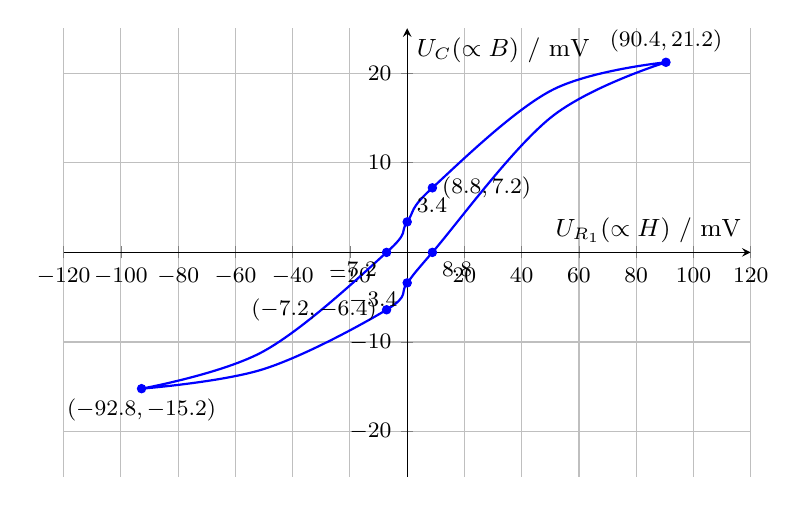
\begin{tikzpicture}
        \begin{axis}[
            axis lines=middle,
            xlabel={$U_{R_1}(\propto H)$ / mV},
            ylabel={$U_C(\propto B)$ / mV},
            xmin=-120, xmax=120,
            ymin=-25, ymax=25,
            grid=both,
            width=0.85\textwidth,
            height=0.6\textwidth,
            tick label style={font=\footnotesize},
            label style={font=\small},
            % smooth cycle? No, just close it at the end
        ]
        
        \addplot[smooth, thick, blue, tension=0.6] coordinates {
            % Upper Branch (Decreasing H) - S+ to S-
            (90.4, 21.2)      % Saturation +
            (50, 18)          % Aux: Knee region
            (8.80, 7.20)      % Data: Hc+
            (0, 3.4)          % Data: Br+
            (-7.20, 0)        % Data: Hc-
            (-50, -11)        % Aux: Approach Saturation
            (-92.8, -15.2)    % Saturation -
            
            % Lower Branch (Increasing H) - S- to S+
            (-92.8, -15.2)    % Saturation -   
            (-50, -13)        % Aux: Knee region
            (-7.20, -6.40)    % Data: Hc- (Vertical pair)
            (0, -3.4)         % Data: Br-
            (8.80, 0)         % Data: Hc+ (Vertical pair)
            (50, 15)          % Aux: Approach Saturation
            (90.4, 21.2)      % Back to Saturation +
        };
        
        % Data Points Markers (Optional circle markers for actual data)
        \addplot[only marks, mark=*, mark size=1.5pt, blue] coordinates {
            (90.4, 21.2)
            (8.80, 7.20)
            (0, 3.4)
            (-7.20, 0)
            (-92.8, -15.2)
            (-7.20, -6.40)
            (0, -3.4)
            (8.80, 0)
        };

        % Annotations
        \node[above] at (axis cs:90.4, 21.2) {\footnotesize $(90.4, 21.2)$};
        \node[below] at (axis cs:-92.8, -15.2) {\footnotesize $(-92.8, -15.2)$};
        
        \node[above right] at (axis cs:0, 3.4) {\footnotesize $3.4$};
        \node[below left] at (axis cs:0, -3.4) {\footnotesize $-3.4$};
        
        \node[below left] at (axis cs:-7.20, 0) {\footnotesize $-7.2$};
        \node[below right] at (axis cs:8.80, 0) {\footnotesize $8.8$};

        \node[right] at (axis cs:8.80, 7.20) {\footnotesize $(8.8, 7.2)$};
        \node[left] at (axis cs:-7.20, -6.40) {\footnotesize $(-7.2, -6.4)$};

        \end{axis}
    \end{tikzpicture}
    \caption{频率 $f=100\text{ Hz}$ 时的饱和磁滞回线数据示意图}
    \label{fig:hysteresis_100hz_data}
\end{figure}

\vspace{1em}

(2) 固定信号源幅度，观测并记录饱和磁滞回线随频率的变化规律。

保持 $R_1, R_2C$ 不变，测量并比较 $f=95\text{ Hz}$ 和 $150\text{ Hz}$ 时的 $B_r$ 和 $H_c$。

\begin{table}[h!]
    \centering
    \renewcommand{\arraystretch}{1.5}
    \begin{tabular}{ccc}
        \toprule
         & 95Hz & 150Hz \\ 
        \midrule
        $(B_r)$ & $4.20\text{ mV}$ & $2.48\text{ mV}$ \\
        $(H_c)$ & $9.20\text{ mV}$ & $5.60\text{ mV}$ \\
        \bottomrule
    \end{tabular}
    \caption{不同频率下饱和磁滞回线变化规律}
\end{table}

\begin{enumerate}
    \item[(a)] 本实验观察到的变化规律：随着信号源频率 $f$ 从 $95\text{ Hz}$ 增加到 $150\text{ Hz}$，测得的剩磁 $B_r$（对应 $U_C$）和矫顽力 $H_c$（对应 $U_{R_1}$）均出现明显的下降。
    \item[(b)] 分析上述变化的原因：
    \begin{itemize}
        \item 励磁电流减小：励磁线圈具有电感特性，其阻抗 $Z \approx \omega L$ 随频率升高而增大。在信号源输出电压幅度保持不变的情况下，励磁电流 $i_1$ 减小，导致磁场强度 $H$ 幅值降低，磁化程度减弱。
        \item 积分电路特性：根据公式 $u_C \approx \frac{1}{R_2C} \int u_2 dt$，对于相同的磁感应强度变化率，积分电路的输出电压与频率成反比（$1/f$ 关系）。因此频率升高会导致示波器上观测到的 $u_C$ 信号幅度减小。
        \item 涡流损耗影响：虽然频率升高通常会因涡流损耗增大而使磁滞回线面积变大，但在本实验电路条件下，上述电路参数随频率的变化（阻抗增加和积分电压衰减）占据了主导地位。
    \end{itemize}
\end{enumerate}

\vspace{1em}

(3) 不同积分常量下的动态磁滞回线

在频率 $f=50\text{ Hz}$ 下，比较不同积分常量取值对李萨如图的影响。

固定励磁电流幅度 $I_m=0.1\text{ A}$，$R_1=2.0\Omega$，改变积分常量 $R_2C$。调节分别为 $0.01\text{ s}$、$0.05\text{ s}$、$0.5\text{ s}$。
下面为不同积分常量下李萨如图形的示意图。
\begin{figure}[H]
    \centering
    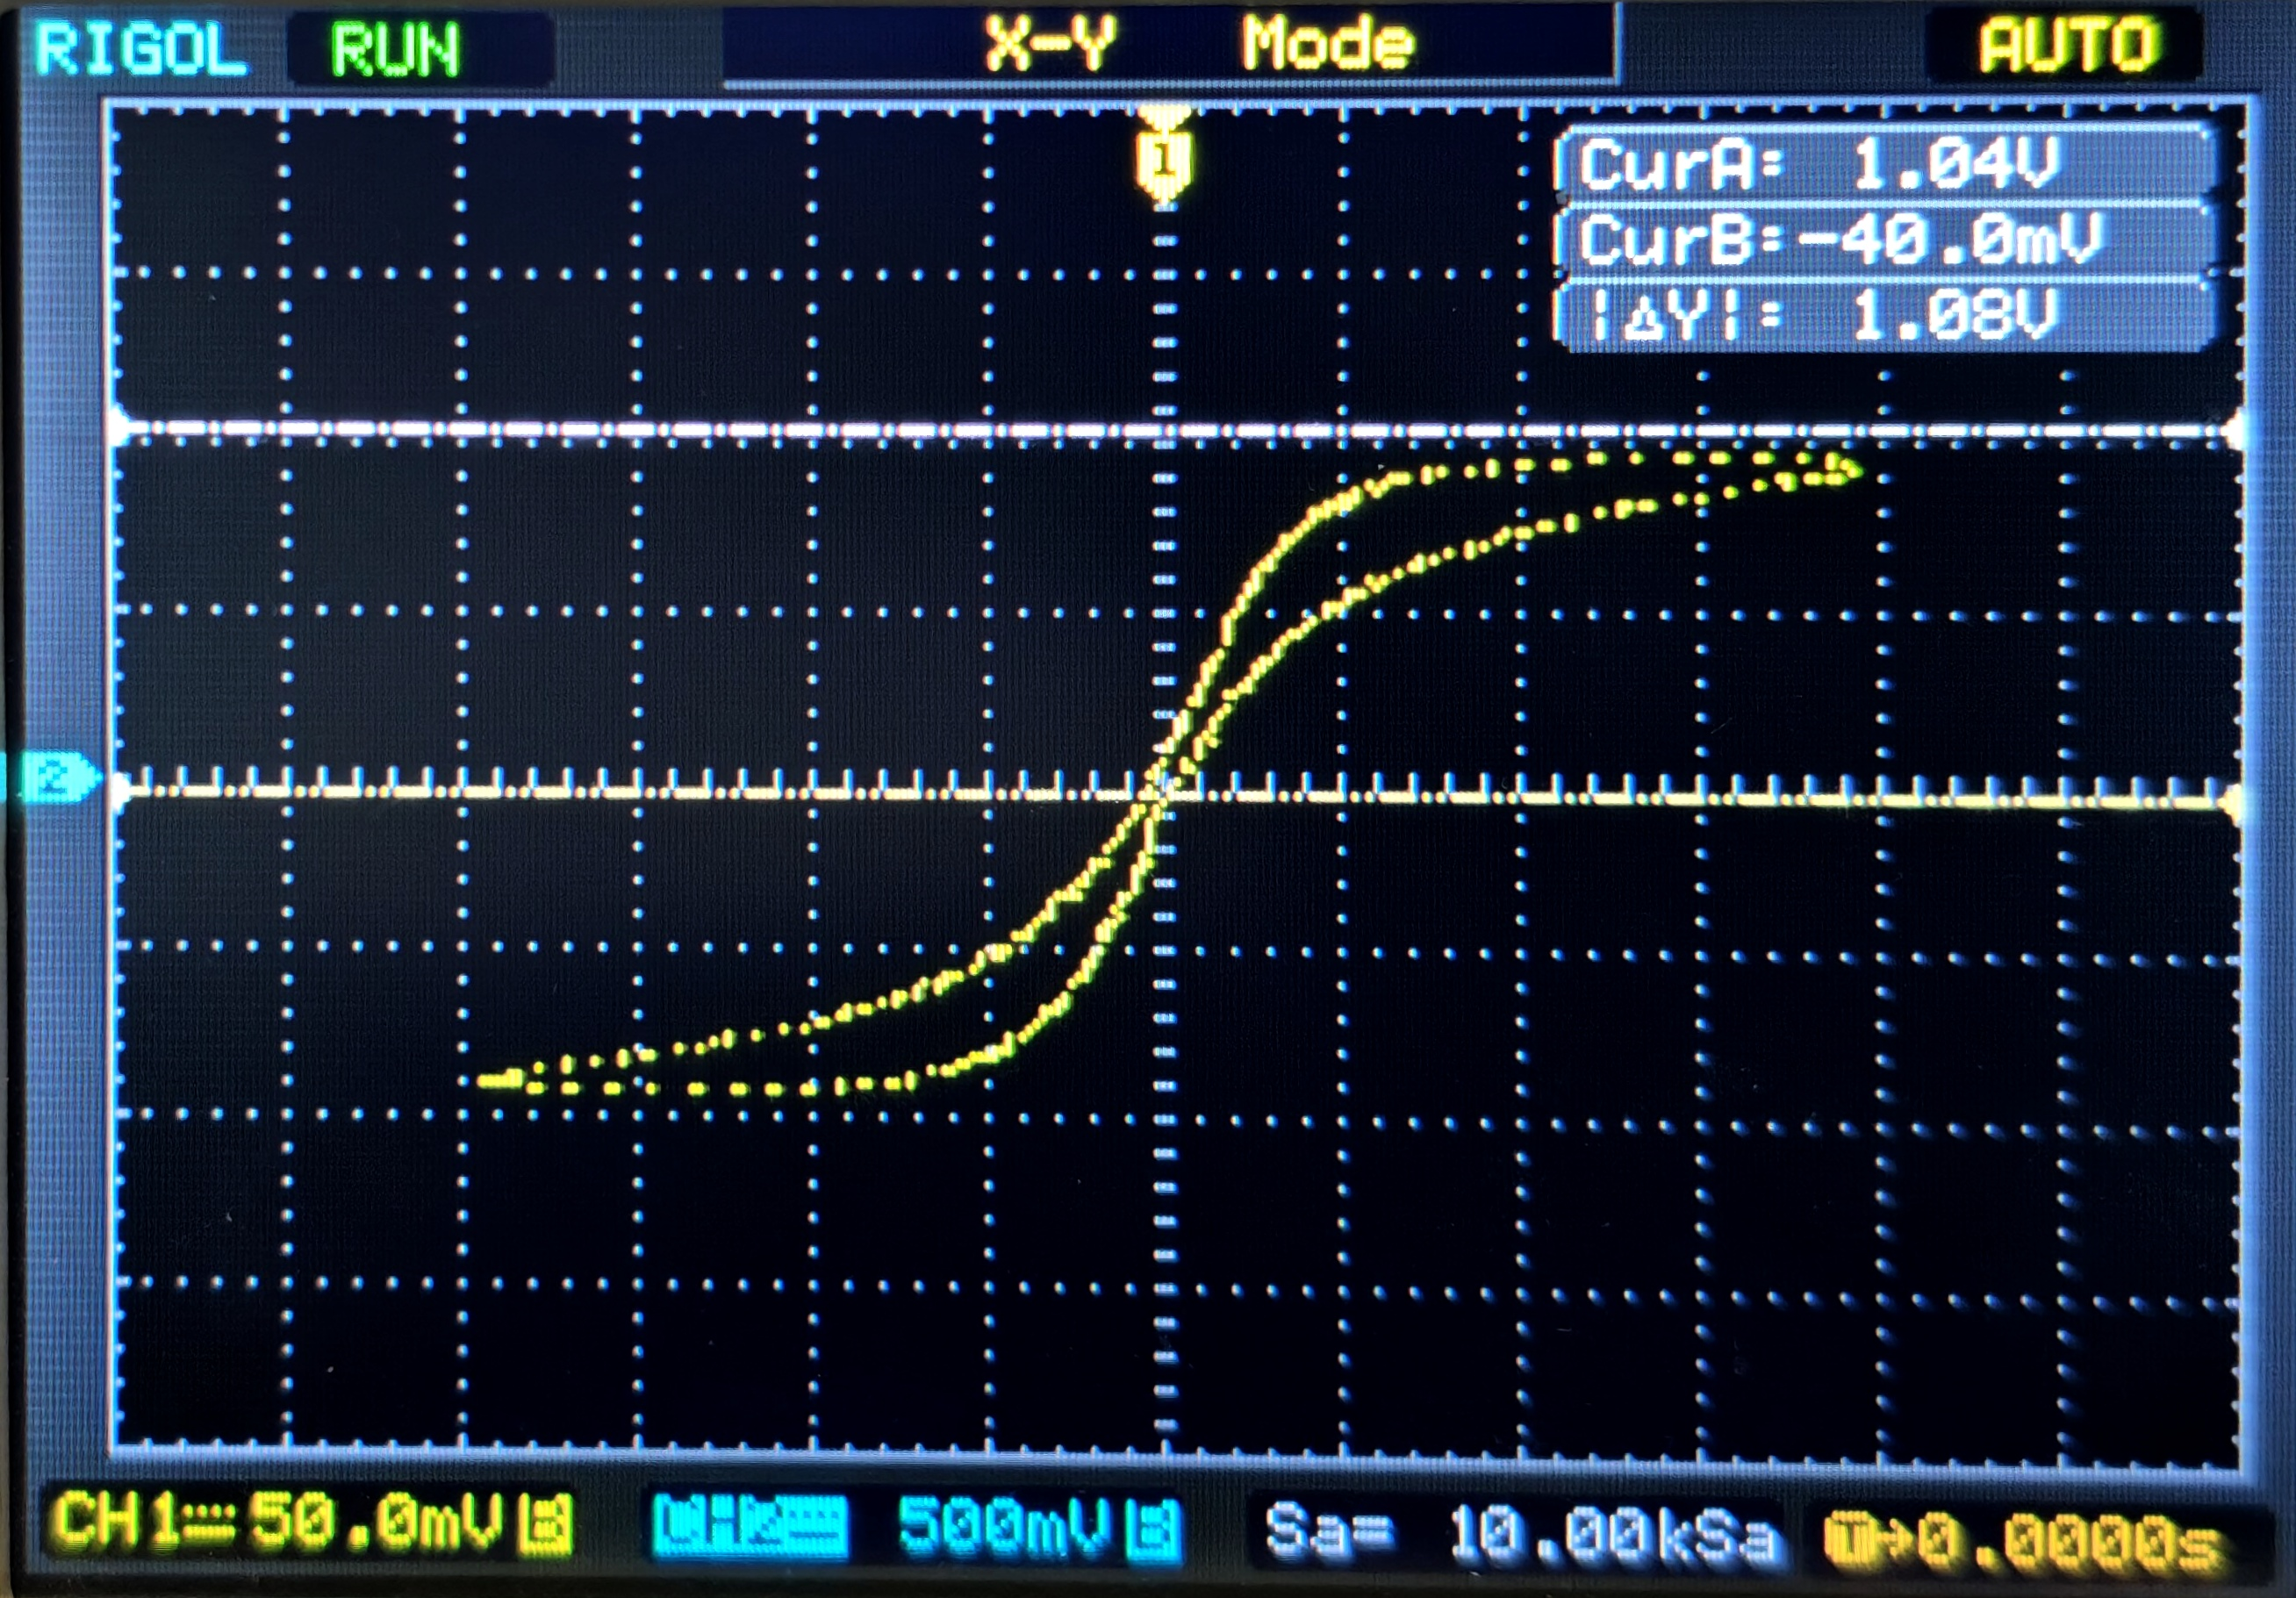
\includegraphics[width=0.9\textwidth]{t_0.01.jpg}
    \caption{T=0.01s 下李萨如图形示意图}
    \label{fig:integral_constant_0.01}
\end{figure}

\begin{figure}[H]
    \centering
    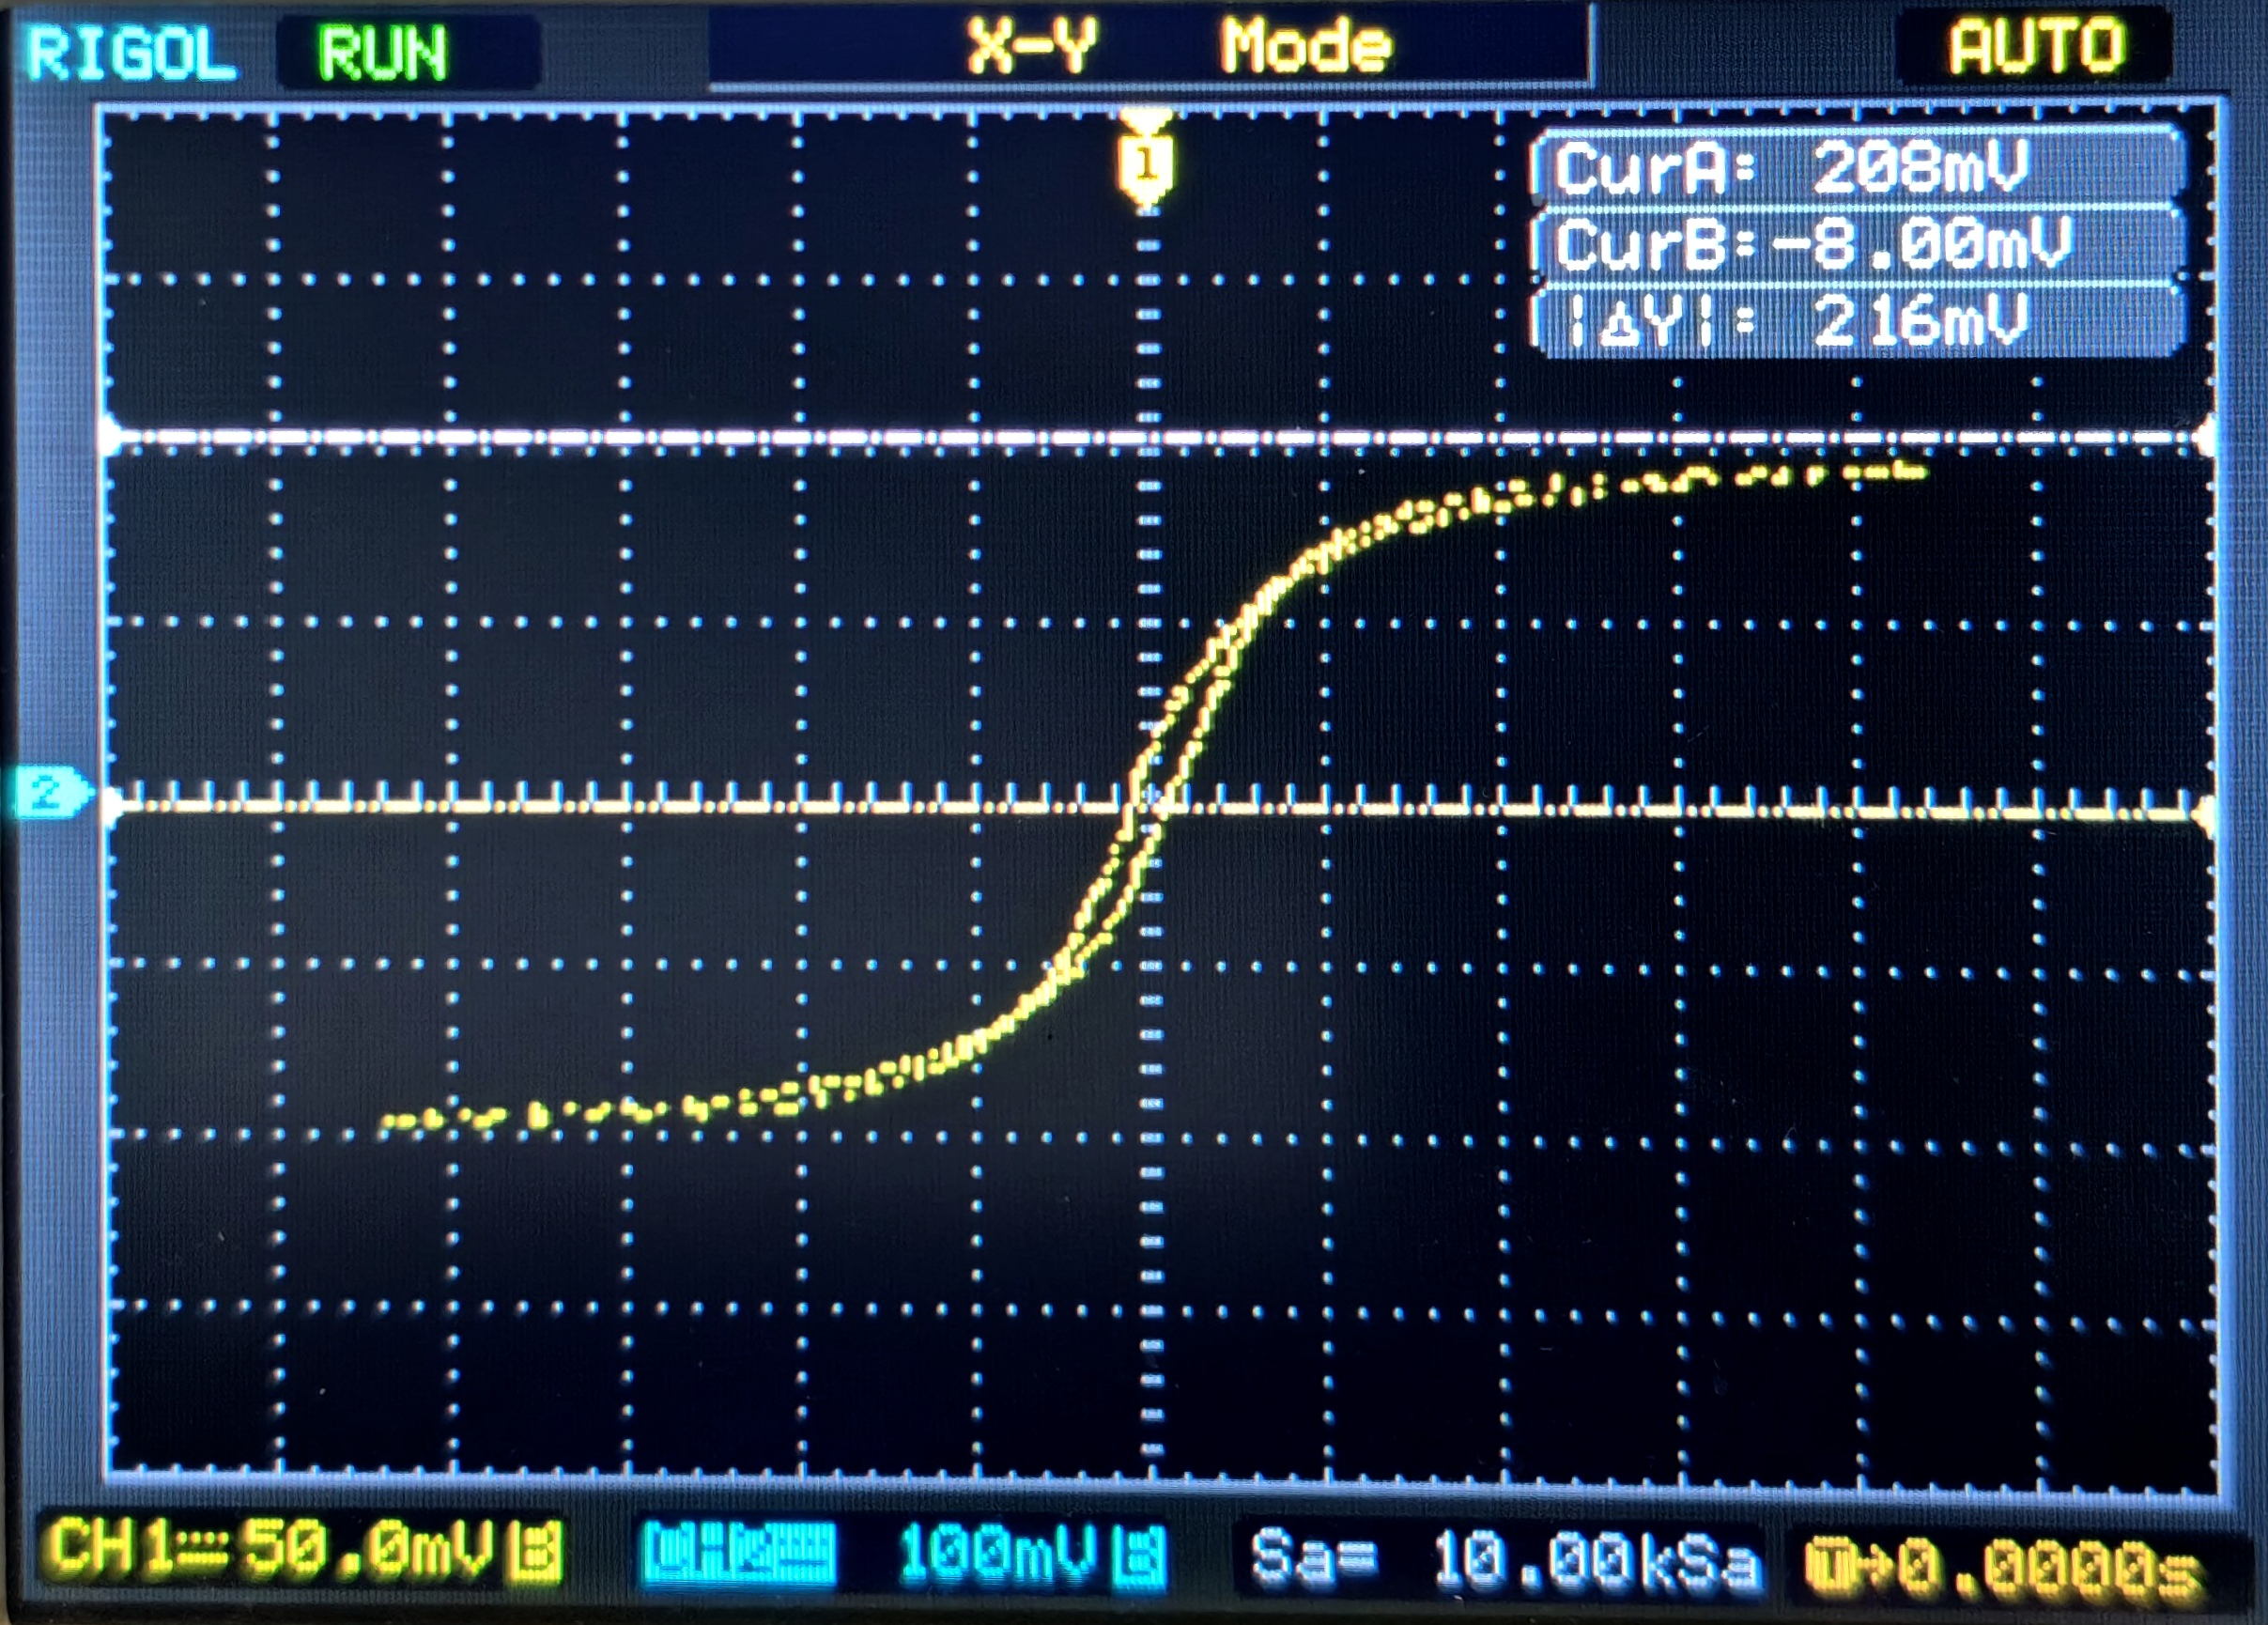
\includegraphics[width=0.9\textwidth]{t_0.05.jpg}
    \caption{T=0.05s 下李萨如图形示意图}
    \label{fig:integral_constant_0.05}
\end{figure}

\begin{figure}[H]
    \centering
    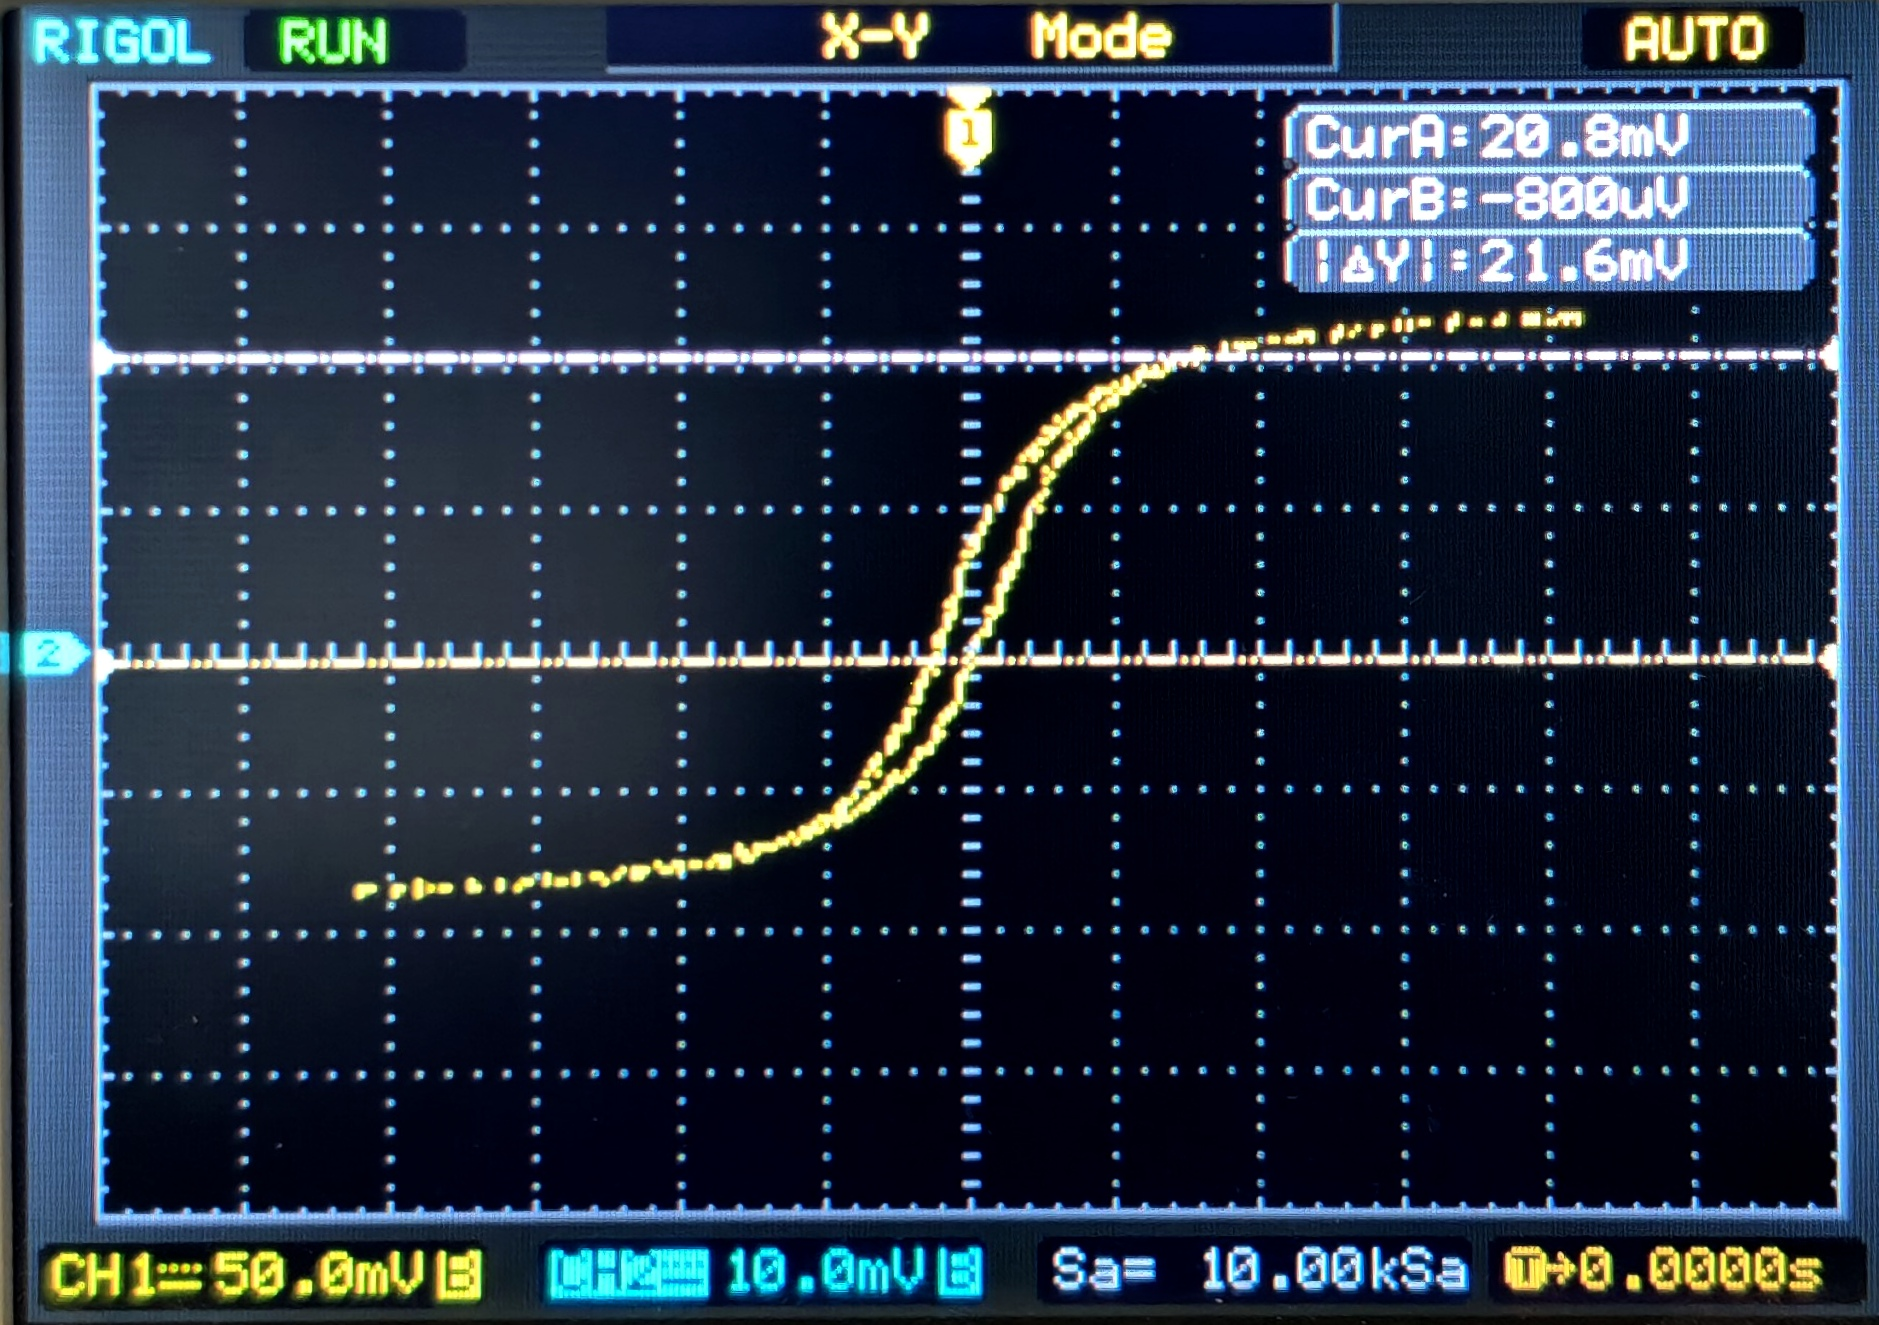
\includegraphics[width=0.9\textwidth]{t_0.5.jpg}
    \caption{T=0.5s 下李萨如图形示意图}
    \label{fig:integral_constant_0.5}
\end{figure}



\noindent (a) 为什么积分常量会影响李萨如图形的形状？\\
\textbf{回答：} 积分常量 $\tau = R_2C$ 决定了积分电路的传递函数和输出电压 $u_C$ 的幅值。根据原理公式 $u_C \approx \frac{1}{R_2C} \int u_2 dt = \frac{N_2 S}{R_2 C} B$，积分常量直接作为分母影响 $u_C$ 的纵向比例，从而改变图形的宽窄胖瘦。此外，RC积分电路正常工作的条件是 $\tau \gg T$（$T$ 为信号周期）。若 $\tau$ 取值过小，积分条件不满足，输出信号不再与磁感应强度 $B$ 成正比，会导致图形发生明显的相位移动和波形畸变；若 $\tau$ 过大，则输出信号极其微弱，导致信噪比降低，图形缩小。

\noindent (b) 积分常量是否会影响真实的磁滞回线的形状？\\
\textbf{回答：} 不会。积磁常量 $\tau = R_2C$ 只是测量仪器的一部分参数，它只影响我们观测到的电压信号（即磁滞回线在示波器上的“投影”或比例）。铁磁材料真实的 $B-H$ 关系是由材料本身的性质（如磁畴结构、杂质、应力等）以及外加磁场频率决定的，属于材料的固有物理特性，不会随外部 RC 电路元件参数的选择而改变。数据处理时通过公式(2)抵消了 $R_2C$ 的影响，理论上应得到一致的 $B-H$ 图。

\subsubsection{测量样品 1（铁氧体）的动态磁化曲线}

(1) 在 $f=100\text{ Hz}$ 时，取 $R_1=2.0\ \Omega$，$R_2=50\text{ k}\Omega$，$C=10.0\ \mu\text{F}$。实验数据在表格 \ref{table:dynamic_hysteresis_loop}，动态磁化曲线如图 \ref{fig:dynamic_mag}，振幅磁导率随磁场变化曲线如图 \ref{fig:permeability_curve}。

\begin{table}[h!]
    \centering
    \caption{动态磁化曲线测量数据}
    \label{table:dynamic_hysteresis_loop}
    \renewcommand{\arraystretch}{1.3}
    \setlength{\tabcolsep}{2pt}
    \resizebox{\textwidth}{!}{
    \begin{tabular}{cccccccccccccccc}
        \toprule
        序号 & 1 & 2 & 3 & 4 & 5 & 6 & 7 & 8 & 9 & 10 & 11 & 12 & 13 & 14 & 15 \\ 
        \midrule
        $(2 \delta H)/\text{mV}$ & 6.60 & 24.0 & 30.4 & 33.6 & 41.8 & 62.0 & 75.6 & 85.2 & 98.4 & 111 & 125 & 138 & 153 & 163 & 180 \\
        $(2 \delta B)/\text{mV}$ & 2.80 & 9.00 & 10.6 & 12.2 & 15.4 & 21.6 & 25.2 & 28.8 & 30.8 & 32.0 & 33.6 & 34.8 & 36.0 & 36.8 & 37.6 \\
        \bottomrule
    \end{tabular}
    }
\end{table}

\begin{figure}[H]
    \centering
    \begin{tikzpicture}
        \begin{axis}[
            width=0.85\textwidth,
            height=0.6\textwidth,
            xlabel={$U_{R_1}(\propto 2 \delta H)$ / mV},
            ylabel={$U_C(\propto 2 \delta B)$ / mV},
            grid=both,
            minor tick num=1,
            legend pos=south east,
            title={动态磁化曲线 ($B_m - H_m$)},
            mark size=2pt
        ]
        \addplot[
            color=red,
            mark=*,
            smooth,
            tension=0.5
        ] coordinates {
            (0,0) % Origin
            (6.60, 2.80)
            (24.0, 9.0)
            (30.4, 10.6)
            (33.6, 12.2)
            (41.8, 15.4)
            (62.0, 21.6)
            (75.6, 25.2)
            (85.2, 28.8)
            (98.4, 30.8)
            (111, 32.0)
            (125, 33.6)
            (138, 34.8)
            (153, 36.0)
            (163, 36.8)
            (180, 37.6)
        };
        \legend{实验测量点}
        \end{axis}
    \end{tikzpicture}
    \caption{铁氧体样品动态磁化曲线}
    \label{fig:dynamic_mag}
\end{figure}

\begin{figure}[H]
    \centering
    \begin{tikzpicture}
        \begin{axis}[
            width=0.85\textwidth,
            height=0.6\textwidth,
            xlabel={$U_{R_1}(\propto H_m)$ / mV},
            ylabel={振幅磁导率 $\mu_m(\propto B_m/H_m)$},
            grid=both,
            minor tick num=1,
            title={振幅磁导率随磁场变化曲线 ($\mu_m - H_m$)},
            mark size=2pt
        ]
        \addplot[
            color=blue,
            mark=square*,
            smooth,
            tension=0.5
        ] coordinates {
            (6.60, 0.4242)
            (24.0, 0.3750)
            (30.4, 0.3487)
            (33.6, 0.3631)
            (41.8, 0.3684)
            (62.0, 0.3484)
            (75.6, 0.3333)
            (85.2, 0.3380)
            (98.4, 0.3130)
            (111, 0.2883)
            (125, 0.2688)
            (138, 0.2522)
            (153, 0.2353)
            (163, 0.2258)
            (180, 0.2089)
        };
        \end{axis}
    \end{tikzpicture}
    \caption{振幅磁导率 $\mu_m$ 随磁场强度 $H_m$ 的变化曲线}
    \label{fig:permeability_curve}
\end{figure}

\noindent (3) 确定起始磁导率：

根据起始磁化曲线的定义，起始磁导率 $\mu_i$ 为磁场强度 $H \to 0$ 时磁感应强度 $B$ 与 $H$ 之比的极限值。在实验测量中，由于无法做到真正的 $H=0$，通常取磁场强度极小时的振幅磁导率作为近似。

根据 $\mu_m - H_m$ 曲线及测量数据，取第一个测量点（最小磁场强度点）：
$U_{R_1} = 6.60\text{ mV}, U_C = 2.80\text{ mV}$。

利用相对磁导率公式：
\begin{equation}
    \mu_r = \frac{R_2 C l R_1}{N_1 N_2 S \mu_0} \cdot \frac{u_C}{u_{R_1}}
\end{equation}
代入样品 1 参数：$l=0.130\text{ m}, S=1.24\times 10^{-4}\text{ m}^2, N_1=150, N_2=150$，以及电路参数 $R_1=2.0\ \Omega, R_2=50\text{ k}\Omega, C=10.0\ \mu\text{F}$：
\begin{equation}
    \mu_i \approx \frac{50\times 10^3 \times 10\times 10^{-6} \times 0.130 \times 2.0}{150 \times 150 \times 1.24\times 10^{-4} \times 4\pi \times 10^{-7}} \times \frac{2.80}{6.60} \approx 37090 \times 0.4242 \approx 1.57 \times 10^4
\end{equation}
由此确定该铁氧体样品的起始相对磁导率约为 $1.57 \times 10^4$。




\subsubsection{观察不同频率下样品 2（硅钢）的动态磁滞回线}

参数调至 $R_1=2.0\ \Omega, R_2=50\text{ k}\Omega, C=10.0\ \mu\text{F}$。在给定交变磁场幅度 $H_m=400\text{ A/m}$ 下，测量三种频率下的 $B_m, B_r, H_c$。
测量结果如表\ref{tab:diff_para}所示：
\begin{table}[h!]
    \centering
    \caption{不同频率下的磁滞参数}
    \label{tab:diff_para}
    \renewcommand{\arraystretch}{1.5}
    \begin{tabular}{cccc}
        \toprule
         & 20Hz & 40Hz & 60Hz \\ 
        \midrule
        $(B_m)$ & $31.2\text{ mV}$ & $30.4\text{ mV}$ & $30.4\text{ mV}$ \\
        $(B_r)$ & $16.8\text{ mV}$ & $17.6\text{ mV}$ & $18.4\text{ mV}$ \\
        $(H_c)$ & $96\text{ mV}$ & $120\text{ mV}$ & $128\text{ mV}$ \\
        \bottomrule
    \end{tabular}
\end{table}

\subsubsection{测量样品 1（铁氧体）在不同直流偏置磁场下的可逆磁导率}

取 $f=100\text{ Hz}$。电路参数设置为：$R_1=2.0\ \Omega, R_2=20\text{ k}\Omega, C=2.0\ \mu\text{F}$。直流偏置磁场从 0 到 $H_s$ 单调增加（缓慢增加）。测量 10 组磁滞回线小线段的斜率。把电流换算成磁场强度 $H$，并绘制可逆磁导率随外场强度的变化曲线 $\mu_i-H$。
这里按照实验老师的要求，只需测量第一象限$\Delta X $和$\Delta Y $再计算即可。
\begin{table}[h!]
    \centering
    \caption{可逆磁导率测量数据}
    \renewcommand{\arraystretch}{1.4}
    \setlength{\tabcolsep}{4pt}
    \begin{tabular}{ccccccccccc}
        \toprule
        & 1 & 2 & 3 & 4 & 5 & 6 & 7 & 8 & 9 & 10 \\ 
        \midrule
        电流 $I$ (mA) & 1.40 & 2.08 & 3.00 & 4.76 & 6.90 & 8.85 & 10.1 & 19.0 & 22.8 & 53.0 \\
        端点坐标 $\Delta H$ (mV) & 2.80 & 4.16 & 6.00 & 9.52 & 13.8 & 17.7 & 20.2 & 38.0 & 45.6 & 106 \\
        端点坐标 $\Delta B$ (mV) & 6.08 & 6.80 & 6.04 & 7.28 & 7.28 & 6.48 & 5.36 & 6.64 & 6.32 & 10.5 \\
        磁场强度 $H$ (A/m) & 21.5 & 32.0 & 46.2 & 73.2 & 106 & 136 & 155 & 292 & 351 & 815 \\
        可逆磁导率 $\mu_i (\times 10^3)$ & 15.7 & 11.8 & 7.28 & 5.53 & 3.81 & 2.65 & 1.92 & 1.26 & 1.00 & 0.72 \\
        \bottomrule
    \end{tabular}
\end{table}

\begin{figure}[h!]
    \centering
    \begin{tikzpicture}
        \begin{axis}[
            xlabel={磁场强度 $H$ (A/m)},
            ylabel={可逆磁导率 $\mu_i$},
            grid=major,
            width=10cm,
            height=7cm,
            mark size=2pt
        ]
        \addplot+[smooth, mark=o] coordinates {
            (21.5, 15700) 
            (32.0, 11819) 
            (46.2, 7278) 
            (73.2, 5529) 
            (106.2, 3814) 
            (136.2, 2647) 
            (155.4, 1919) 
            (292.3, 1263) 
            (350.8, 1002) 
            (815.4, 716)
        };
        \end{axis}
    \end{tikzpicture}
    \caption{可逆磁导率 $\mu_i$ 随磁场强度 $H$ 的变化曲线}
    \label{fig:mu_i_curve}
\end{figure}

\paragraph{分析与讨论}
由图 \ref{fig:mu_i_curve} 及实验数据可见，随着直流偏置磁场 $H$ 的增大，铁氧体样品的可逆磁导率 $\mu_i$ 呈现单调下降的趋势。
\begin{enumerate}
    \item 在低直流偏置磁场下（$H < 50\text{ A/m}$），$\mu_i$ 维持在较高数值（约 $1.5\times 10^4$）。此时材料尚未饱和，磁畴壁在微小交流信号驱动下容易发生可逆位移，对交流信号有很强的响应。
    \item 随着直流偏置磁场逐渐增加，材料内部磁矩逐渐趋向于沿外场方向排列，材料开始接近磁饱和状态。此时，磁畴壁受到更强的钉扎作用或已移动至极限位置，微小交流场引起的磁感应强度变化量 $\Delta B$ 变小，导致可逆磁导率迅速衰减。
    \item 实验数据显示，当 $H$ 达到 $800\text{ A/m}$ 时，$\mu_i$ 仅余初始值的约 $5\%$。这一结果验证了铁磁材料在静态偏置磁场作用下，其增量（可逆）磁导率会随磁化强度的增加而显著降低的物理性质。
\end{enumerate}

\subsection{用霍尔传感器测量铁磁材料（准）静态磁滞回线}

\subsubsection{测量样品的起始磁化曲线}

将霍尔传感器置于磁场均匀区的中央。取 20 个采样点，测量样品的起始磁化曲线。
实验原始数据如表\ref{tab:start}

\begin{table}[H]
    \centering
    \caption{起始磁化曲线测量数据}
    \label{tab:start}
    \renewcommand{\arraystretch}{1.3} % 增加行高，使表格更清晰
    \setlength{\tabcolsep}{4pt}       % 调整列间距以适应页面宽度
    \small                            % 稍微减小字号以容纳8列数据
    \begin{tabular}{cccc}
        \toprule
        $I$ & $B$ & $H$ & 修正 $H$ \\
        (\si{\milli\ampere}) & (\si{\milli\tesla}) & (\si{\ampere\per\meter}) & (\si{\ampere\per\meter}) \\
        \midrule
        50.0   & 12.0  & 416 & 337 \\
        103.8  & 27.8  & 865 & 680 \\
        150.1  & 51.2  & 1250& 911 \\
        200.3  & 78.2  & 1669& 1150\\
        250.1  & 107.7 & 2084& 1369\\
        300.6  & 141.7 & 2505& 1565\\
        350.5  & 175.6 & 2920& 1756\\
        400.4  & 206.1 & 3336& 1969\\
        450.6  & 230.7 & 3755& 2225\\
        500.4  & 260.6 & 4170& 2441\\
        553.1 & 296.2 & 4609 & 2644 \\
        600.3 & 319.1 & 5002 & 2886 \\
        650.2 & 339.5 & 5400 & 3128 \\
        \bottomrule
    \end{tabular}
\end{table}

\begin{figure}[H]
    \centering
    \begin{tikzpicture}
        \begin{axis}[
            width=0.8\textwidth,
            height=0.6\textwidth,
            xlabel={磁场强度 $H$ (修正) [\si{\ampere\per\meter}]},
            ylabel={磁感应强度 $B$ [\si{\milli\tesla}]},
            grid=both,
            minor tick num=1,
            title={模具钢起始磁化曲线},
            mark size=2pt,
            xmin=0, xmax=3500,
            ymin=0, ymax=350
        ]
        \addplot[
            color=blue,
            mark=*,
            smooth,
            tension=0.3
        ] coordinates {
            (0,0) (337.1,12.0) (680.6,27.8) (911.3,51.2) (1150.6,78.2) (1370.0,107.7) (1565.3,141.7) (1756.3,175.6) (1969.9,206.1) (2225.1,230.7) (2441.8,260.6) (2644.9,296.2) (2886.4,319.1) (3128.6,339.5)
        };
        \end{axis}
    \end{tikzpicture}
    \caption{模具钢的起始磁化曲线 ($B-H$)}
    \label{fig:initial_mag_curve}
\end{figure}

\subsubsection{测量模具钢的磁滞回线}

对样品进行磁锻炼后，磁化线圈的电流从饱和电流 $I_m$ 开始逐步减小到 0，然后将电流反向，电流又从 0 增加到 $-I_m$，重复上述过程，直至回到 $I_m$。每隔约 $50\text{ mA}$ 测一组 $(I_i, B_i)$ 值。
实验数据如表\ref{tab:hysteresis_loop}

\begin{table}[H]
    \centering
    \caption{模具钢磁滞回线测量数据}
    \label{tab:hysteresis_loop}
    \renewcommand{\arraystretch}{1.2} % 适当增加行高
    \setlength{\tabcolsep}{3pt}       % 调整列间距以适应页面宽度
    \tiny                             % 极小字号以容纳大量数据
    \begin{tabular}{cccccccc}
        \toprule
        $I$ & $B$ & $H$ & 修正 $H$ & $I$ & $B$ & $H$ & 修正 $H$ \\
        (\si{\milli\ampere}) & (\si{\milli\tesla}) & (\si{\ampere\per\meter}) & (\si{\ampere\per\meter}) & (\si{\milli\ampere}) & (\si{\milli\tesla}) & (\si{\ampere\per\meter}) & (\si{\ampere\per\meter}) \\
        \midrule
        645.6  & 351.2 & 5380 & 3051 & -645.8 & -356.7 & -5381 & -3016 \\
        595.6  & 344.9 & 4963 & 2676 & -599.8 & -350.7 & -4998 & -2672 \\
        550.4  & 338.5 & 4586 & 2341 & -549.7 & -343.6 & -4580 & -2302 \\
        500.1  & 330.3 & 4167 & 1977 & -500.0 & -335.3 & -4166 & -1943 \\
        447.5  & 320.1 & 3729 & 1606 & -450.1 & -325.5 & -3750 & -1592 \\
        397.3  & 308.0 & 3310 & 1268 & -400.2 & -313.4 & -3335 & -1256 \\
        349.7  & 293.6 & 2914 & 967  & -349.8 & -298.0 & -2915 & -938 \\
        298.3  & 274.1 & 2485 & 668  & -300.0 & -278.9 & -2500 & -650 \\
        249.8  & 251.3 & 2081 & 415  & -250.2 & -255.3 & -2085 & -391 \\
        200.0  & 223.9 & 1666 & 181  & -199.7 & -227.1 & -1664 & -158 \\
        150.0  & 192.9 & 1250 & -29  & -150.0 & -196.0 & -1250 & 49 \\
        100.0  & 159.6 & 833  & -225 & -100.1 & -162.8 & -834  & 245 \\
        50.3   & 124.9 & 419  & -409 & -49.7  & -127.8 & -414  & 433 \\
        0      & 88.2  & 0    & -584 & 0      & -91.1  & 0     & 604 \\
        -49.9  & 51.7  & -415 & -758 & 50.0   & -53.8  & 416   & 773 \\
        -100.4 & 13.4  & -836 & -925 & 100.2  & -17.0  & 835   & 947 \\
        -150.2 & -25.0 & -1251&-1085 & 150.4  & 21.5   & 1253  & 1110 \\
        -199.5 & -63.4 & -1662&-1242 & 200.7  & 60.0   & 1672  & 1274 \\
        -250.4 & -100.5& -2086&-1420 & 252.3  & 97.9   & 2102  & 1453 \\
        -300.1 & -136.3& -2500&-1596 & 300.5  & 132.4  & 2504  & 1626 \\
        -350.2 & -171.6& -2918&-1780 & 352.3  & 168.0  & 2935  & 1821 \\
        -400.6 & -206.1& -3338&-1971 & 400.8  & 201.4  & 3340  & 2004 \\
        -450.9 & -239.4& -3757&-2169 & 451.9  & 234.6  & 3765  & 2210 \\
        -501.4 & -270.7& -4178&-2383 & 501.3  & 264.7  & 4177  & 2422 \\
        -550.0 & -298.4& -4583&-2604 & 551.8  & 293.3  & 4598  & 2653 \\
        -600.1 & -324.6& -5000&-2848 & 599.7  & 317.8  & 4997  & 2890 \\
        -645.8 & -346.0& -5381&-3087 & 645.9  & 350.3  & 5382  & 3059 \\
        \bottomrule
    \end{tabular}
\end{table}

\begin{figure}[H]
    \centering
    \begin{tikzpicture}
        \begin{axis}[
            width=0.85\textwidth,
            height=0.65\textwidth,
            xlabel={磁场强度 $H$ (修正) [\si{\ampere\per\meter}]},
            ylabel={磁感应强度 $B$ [\si{\milli\tesla}]},
            grid=both,
            title={模具钢静态磁滞回线},
            mark size=1.5pt
        ]
        \addplot[
            color=red,
            mark=*,
            smooth,
            tension=0.5
        ] coordinates {
            (3051.0,351.2) (2676.1,344.9) (2341.9,338.5) (1977.1,330.3) (1606.4,320.1) (1268.3,308.0) (967.2,293.6) (668.2,274.1) (415.2,251.3) (181.9,223.9) (-29.2,192.9) (-225.0,159.6) (-409.1,124.9) (-584.9,88.2) (-758.7,51.7) (-925.5,13.4) (-1085.9,-25.0) (-1242.1,-63.4) (-1420.2,-100.5) (-1597.0,-136.3) (-1780.4,-171.6) (-1971.6,-206.1) (-2169.9,-239.4) (-2383.2,-270.7) (-2604.5,-298.4) (-2848.3,-324.6) (-3087.2,-346.0) (-3016.2,-356.7) (-2672.7,-350.7) (-2302.3,-343.6) (-1943.1,-335.3) (-1592.3,-325.5) (-1256.7,-313.4) (-938.8,-298.0) (-650.5,-278.9) (-392.0,-255.3) (-158.2,-227.1) (49.8,-196.0) (245.4,-162.8) (433.3,-127.8) (604.1,-91.1) (773.4,-53.8) (947.7,-17.0) (1110.8,21.5) (1274.6,60.0) (1453.3,97.9) (1626.2,132.4) (1821.7,168.0) (2004.4,201.4) (2210.1,234.6) (2422.2,264.7) (2653.3,293.3) (2890.0,317.8) (3059.5,350.3)
        };
        \end{axis}
    \end{tikzpicture}
    \caption{模具钢的静态磁滞回线 ($B-H$)}
    \label{fig:static_hysteresis_loop}
\end{figure}

\subsubsection{结果分析与讨论}

\paragraph{1. 磁滞回线特征分析}

根据实验数据绘制的模具钢（准）静态磁滞回线显示，该材料具有显著的磁滞现象。
\begin{enumerate}
    \item \textbf{饱和特性}：当励磁电流 $I$ 达到约 \SI{645}{\milli\ampere} 时，磁感应强度 $B$ 达到约 \SI{350}{\milli\tesla}，且随电流增加增长变缓，表明材料已接近饱和状态。
    \item \textbf{剩磁与矫顽力}：
    \begin{itemize}
        \item \textbf{剩磁 $B_r$}：当励磁电流 $I$ 减小至 0 时，样品中仍保留有约 \SI{90}{\milli\tesla} 的磁感应强度。
        \item \textbf{矫顽力 $H_c$}：为了使 $B$ 降为 0，需要施加约 \SI{120}{\milli\ampere} 的反向电流。根据安培环路定律估算（未修正气隙），对应的表观矫顽力较大；经过气隙修正后，不仅磁场强度 $H$ 的数值会显著减小，磁滞回线的形状也会发生“去倾斜”变化，变得更加陡峭。
    \end{itemize}
    \item \textbf{材料对比}：与第一部分实验中的软磁材料（锰锌铁氧体，矫顽力仅约数 \si{\ampere\per\meter}）相比，模具钢的矫顽力（约 \SI{1000}{\ampere\per\meter} 量级）大得多，磁滞回线所包围的面积也显著增大。这说明模具钢属于硬磁材料（或介于软硬之间），具有较大的磁滞损耗，不适合用于高频交变磁场中的变压器铁芯，但适合用于需要一定剩磁保持的场合。
\end{enumerate}

\paragraph{2. 气隙修正的必要性讨论}

本实验中样品存在气隙 $\ell_g = \SI{2.00}{\milli\meter}$。由于气隙中的磁阻远大于铁磁材料本身的磁阻，气隙的存在会产生很强的退磁场。
根据安培环路定律 $H\bar{l} + H_g\ell_g = NI$，其中 $H_g \approx B/\mu_0$。计算表明，气隙项 $H_g\ell_g$ 在总磁动势 $NI$ 中占据了很大比例。如果不进行修正，直接使用 $H = NI/\bar{l}$ 计算，由此得到的磁滞回线将严重向 $H$ 轴倾斜（被剪切），无法真实反映材料本身的磁化特性（即 $B-H$ 关系），而只是反映了包含气隙的整个磁路的特性。修正后的 $H$ 能更准确地代表材料内部的磁场强度。

\paragraph{3. 误差来源分析}

\begin{enumerate}
    \item \textbf{气隙边缘效应}：实验中假设气隙处磁感应强度均匀且 $S_g \approx S$，忽略了边缘漏磁通。实际上气隙处的磁力线会向外扩散，导致测得的 $B$ 值可能略小于材料内部真实的 $B$，修正计算中的 $B/\mu_0$ 项也会引入相应误差。
    \item \textbf{霍尔片位置}：霍尔传感器若未严格置于气隙中心或未与磁力线垂直，测量到的 $B$ 值会偏小。
    \item \textbf{退磁不完全}：起始磁化曲线的测量依赖于样品的完全退磁。如果退磁不彻底，起始点将不在原点，导致整条曲线偏移。
    \item \textbf{磁锻炼影响}：磁滞回线的稳定性依赖于充分的磁锻炼。若循环次数不足，磁畴壁的移动未达到稳定循环状态，测得的数据点可能不闭合或对称性较差。
\end{enumerate}

\section{思考题与解答}

\begin{enumerate}
    \item \textbf{铁磁材料的动态磁滞回线与（准）静态磁滞回线在概念上有什么区别？铁磁材料动态磁滞回线的形状和面积受哪些因素影响？}
    
    \textbf{答：}
    \begin{itemize}
        \item \textbf{概念区别：} 
        \begin{itemize}
            \item \textbf{（准）静态磁滞回线}是在磁场变化极其缓慢（接近直流）的条件下测得的，此时磁感应强度 $B$ 的变化主要由材料内部磁畴的不可逆翻转决定，回路面积仅代表磁滞损耗。
            \item \textbf{动态磁滞回线}是在交变磁场下测得的。在此条件下，铁磁材料内部除了磁滞效应外，还会产生感生电场从而导致涡流（Eddy Current）和磁后效。回路面积代表了总损耗（磁滞损耗 + 涡流损耗 + 剩余损耗）。
        \end{itemize}
        \item \textbf{影响因素：} 
        \begin{itemize}
            \item \textbf{交变磁场的频率 $f$：} 频率越高，涡流效应越显著，损耗增加，导致回线变“胖”（面积增大）。
            \item \textbf{材料的导电率（或电阻率）：} 电阻率越低（如硅钢），涡流越大，动态回线越宽。
            \item \textbf{样品的几何尺寸：} 样品越厚，涡流效应越强。
            \item \textbf{磁场幅值 $H_m$：} 决定了是否达到饱和状态。
        \end{itemize}
    \end{itemize}

    \item \textbf{什么叫做基本磁化曲线？它和起始磁化曲线间有何区别？}
    
    \textbf{答：}
    \begin{itemize}
        \item \textbf{基本磁化曲线：} 对同一铁磁样品，选取不同幅度的交变磁场进行磁化，得到一系列大小不同的稳定的磁滞回线。将这些回线的顶点（即 $(H_m, B_m)$ 点）连接起来所得到的曲线，称为基本磁化曲线。
        \item \textbf{起始磁化曲线：} 将处于完全退磁状态（$B=0, H=0$）的铁磁材料，置于单调增加的磁场中磁化，测得的 $B-H$ 曲线称为起始磁化曲线。
        \item \textbf{区别：} 严格来说两者是不重合的。起始磁化曲线描述的是单次单调磁化过程，而基本磁化曲线描述的是在不同幅值反复磁化达到稳定状态下的顶点轨迹。但在工程应用和一般实验中，常近似认为两者重合。
    \end{itemize}

    \item \textbf{铁氧体和硅钢材料的动态磁化特性各有什么特点？}
    
    \textbf{答：}
    \begin{itemize}
        \item \textbf{铁氧体：} 是一种非金属氧化物磁性材料，具有极高的电阻率（接近绝缘体）。因此在交变磁场下，其内部产生的涡流极小，涡流损耗可以忽略。其动态磁滞回线随频率变化不明显，适合在高频下工作。
        \item \textbf{硅钢：} 是合金金属材料，虽然加入硅增加了电阻率，但相比铁氧体其电阻率仍然较低。在交变磁场下会产生显著的涡流。随着频率升高，涡流损耗急剧增加，导致动态磁滞回线显著变宽（面积增大）。因此硅钢通常制成薄片（叠片）使用，主要适用于低频（如工频 50Hz）环境。
    \end{itemize}

    \item \textbf{动态磁滞回线测量实验中，电路参量应怎样设置才能保证 $u_{R_1} - u_C$ 所形成的李萨如图形正确反映材料动态磁滞回线的形状？}
    
    \textbf{答：}
    实验中通常利用 $R_2C$ 电路作为积分器，将感应电动势（正比于 $dB/dt$）转换为与 $B$ 成正比的电压 $u_C$。
    为了使 $u_C \propto \int u_{in} dt \propto B$，积分电路必须满足积分条件：
    \[ \tau = R_2 C \gg T = \frac{1}{f} \]
    即积分时间常数 $R_2 C$ 必须远大于交变磁场的周期 $T$（通常要求大 10 倍以上）。
    \begin{itemize}
        \item 如果 $R_2 C$ 过小，积分不仅不准确，还会产生较大的幅值和相位误差，导致李萨如图形发生畸变（如不再闭合或形状扭曲），无法正确反映 $B-H$ 关系。
        \item 同时，采样电阻 $R_1$ 应尽量小，以减小对励磁回路电流的影响，保证 $u_{R_1}$ 准确反映磁场强度 $H$。
    \end{itemize}

    \item \textbf{准静态磁滞回线测量实验中，为什么要对样品进行磁锻炼才能获得稳定的饱和磁滞回线？}
    
    \textbf{答：}
    \begin{itemize}
        \item \textbf{原因：} 铁磁材料中磁畴的运动（畴壁位移和磁矩转动）存在类似摩擦的阻力（钉扎效应）。如果样品长期静止或处于某一特定磁化状态，磁畴结构会趋于一种亚稳定状态。
        \item \textbf{目的：} 磁锻炼（即在测量前让电流在 $I_m$ 和 $-I_m$ 之间反复切换多次）的作用是迫使磁畴反复翻转，打破“钉扎”或亚稳态，使畴壁移动达到一种可重复的动态平衡状态。只有经过充分的磁锻炼，材料内部的磁化过程才能稳定下来，从而测得闭合、对称且重复性好的饱和磁滞回线。
    \end{itemize}

\end{enumerate}

\section{预习报告和实验记录原搞}
\begin{figure}
    \centering
    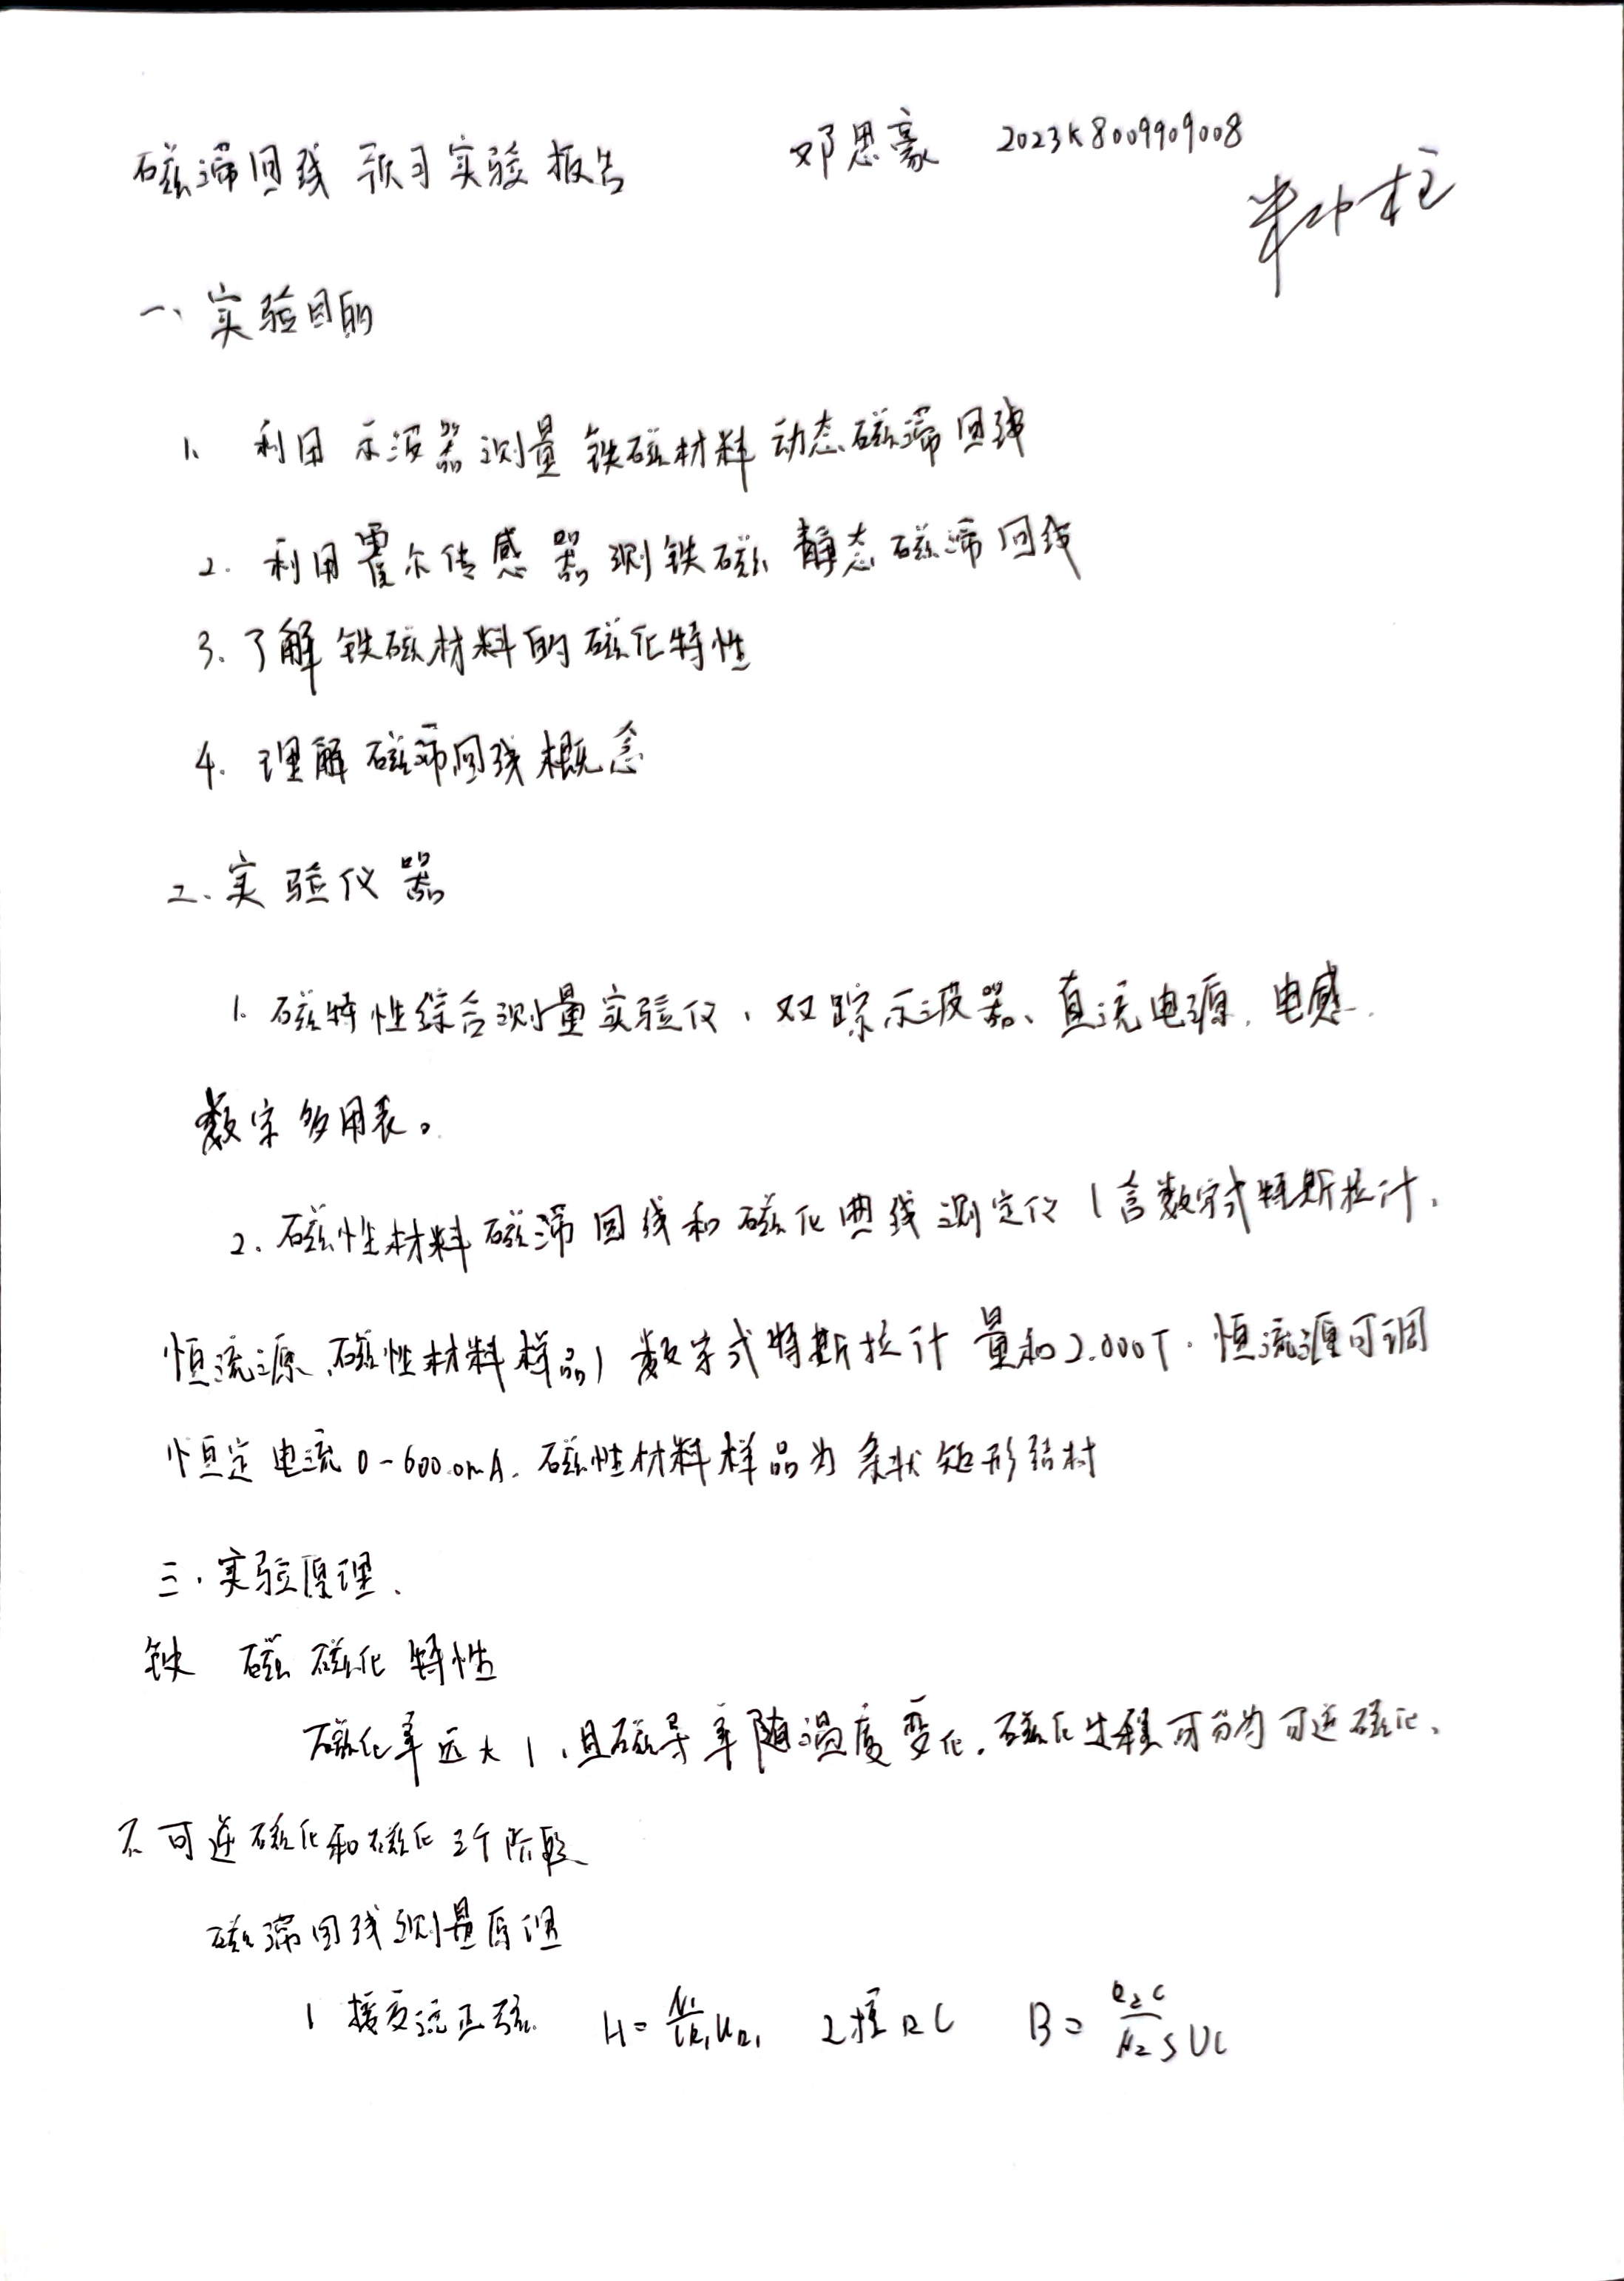
\includegraphics[width=0.9\textwidth]{IMG_20251231_132143.jpg}
    \caption{预习报告原搞}
\end{figure}
\begin{figure}
    \centering
    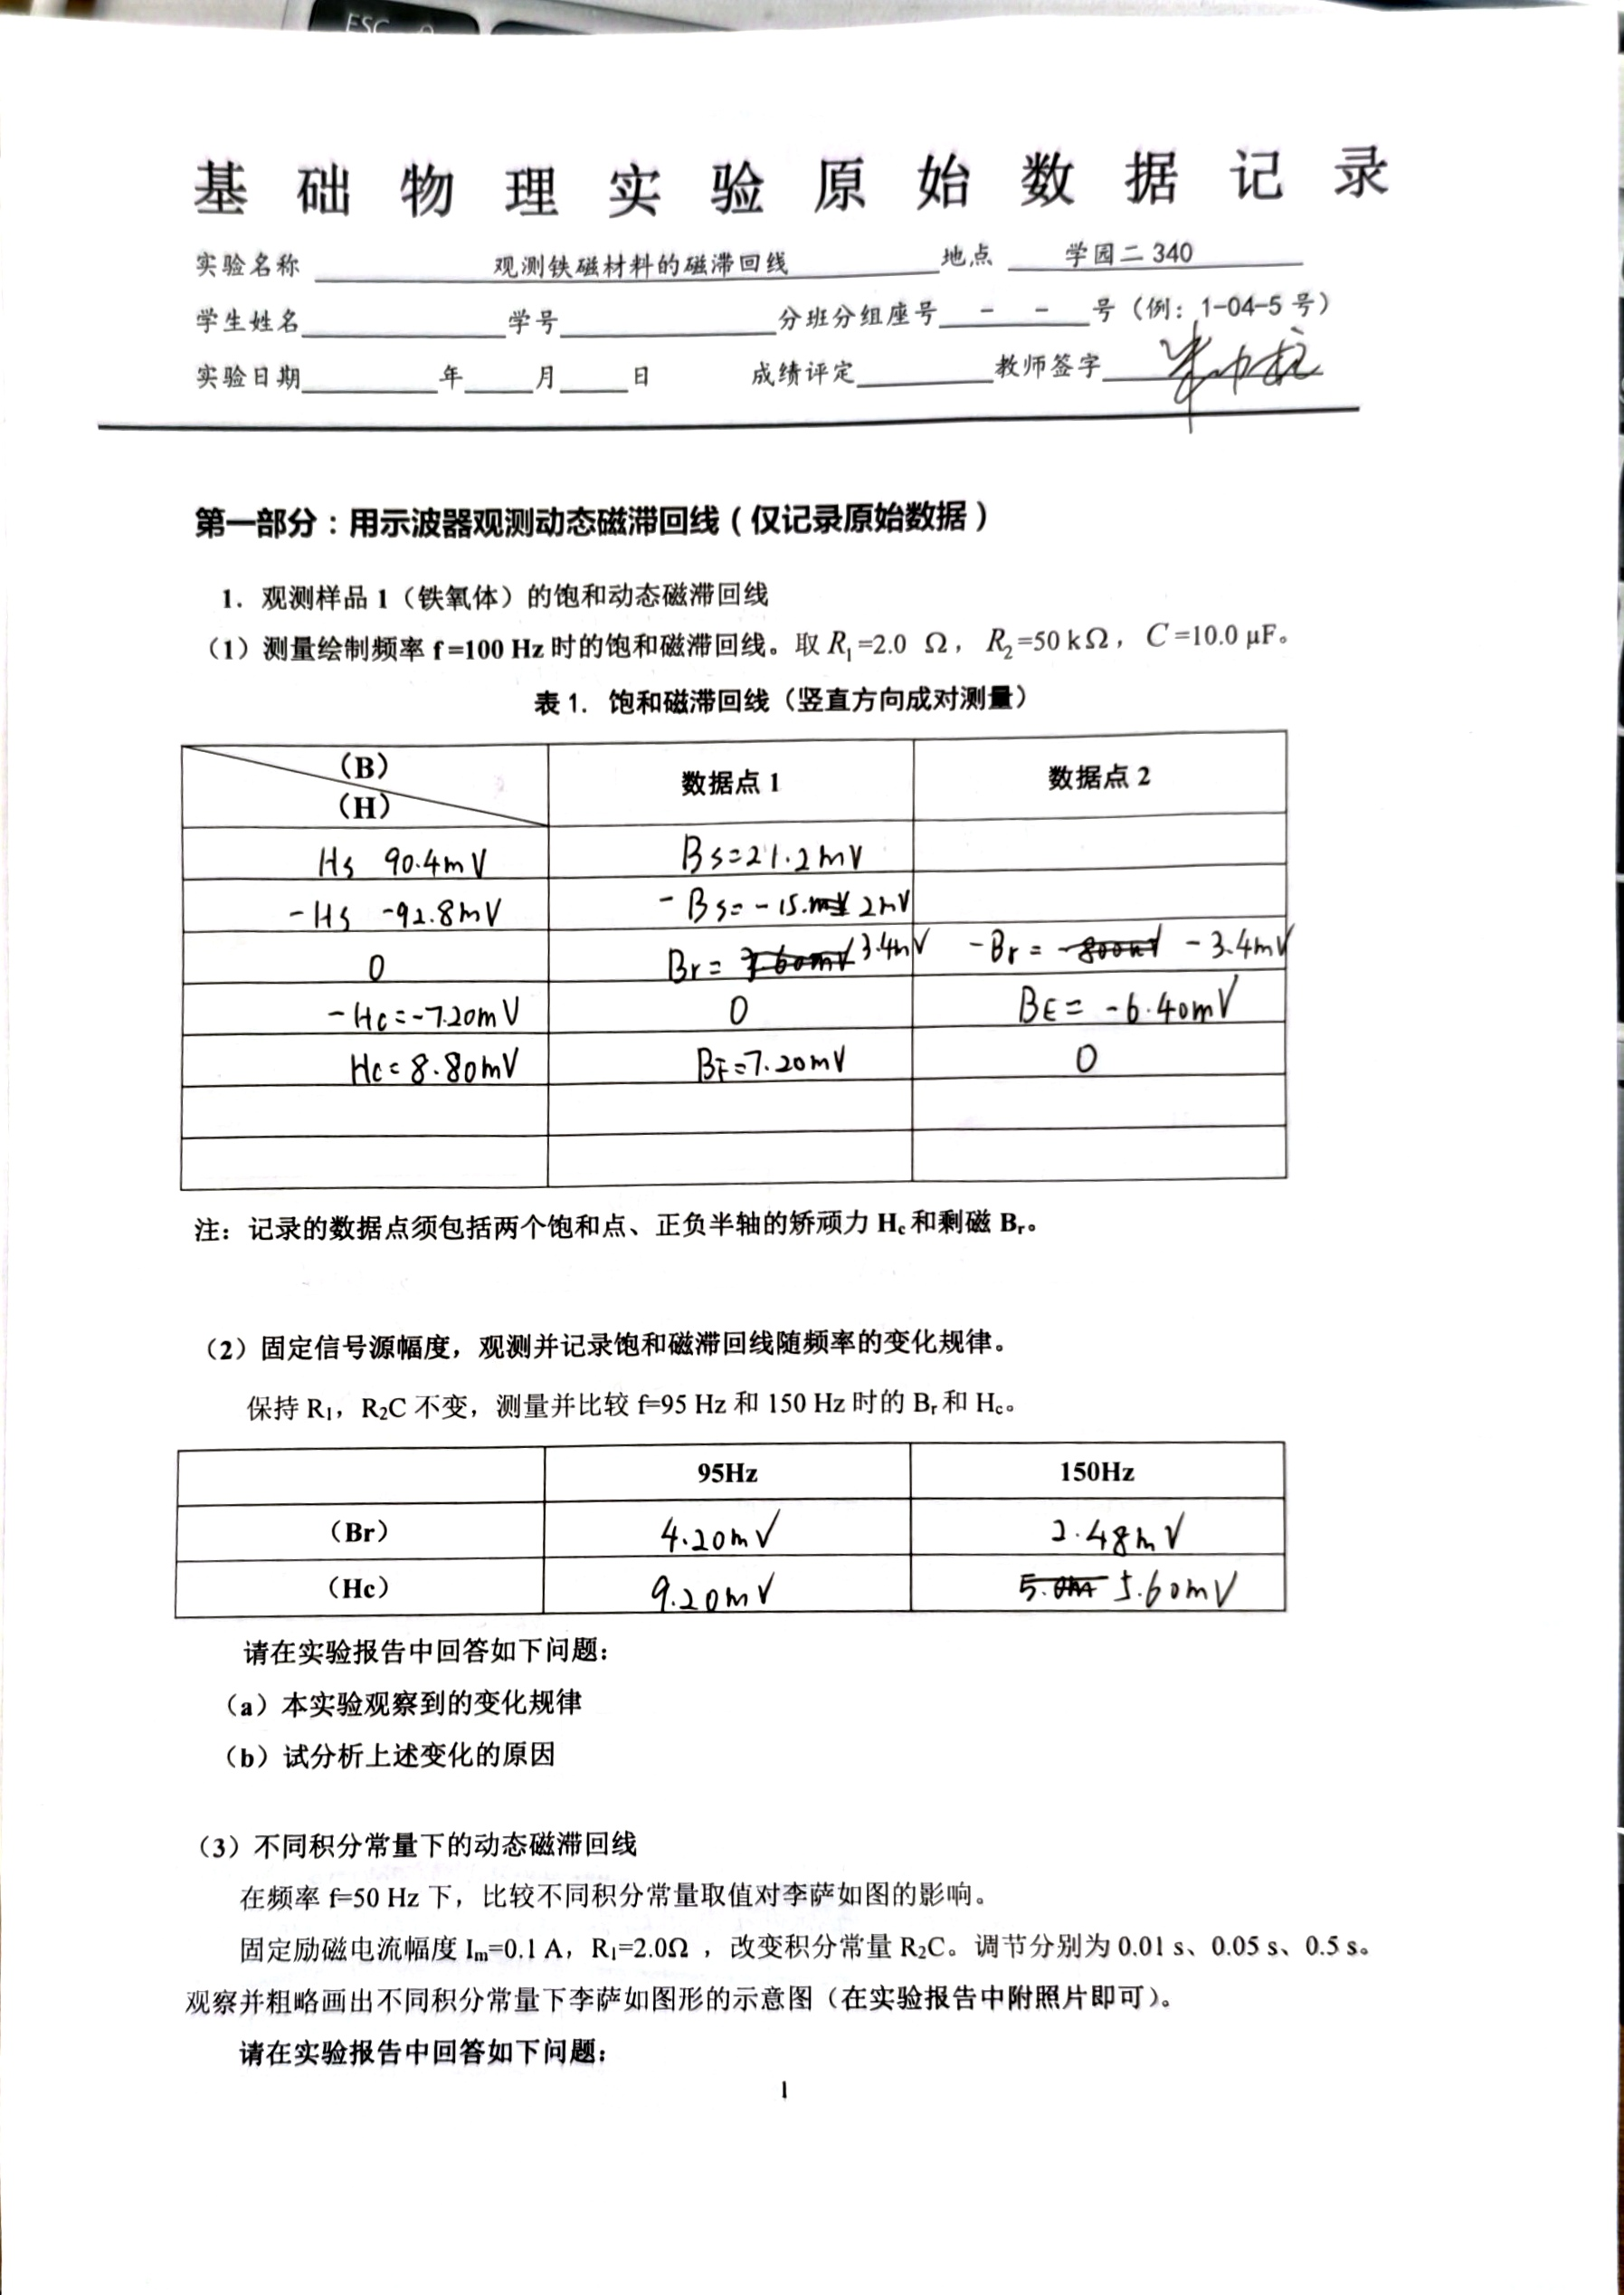
\includegraphics[width=0.9\textwidth]{IMG_20260204_184320.jpg}
    \caption{实验记录1}
\end{figure}
\begin{figure}
    \centering
    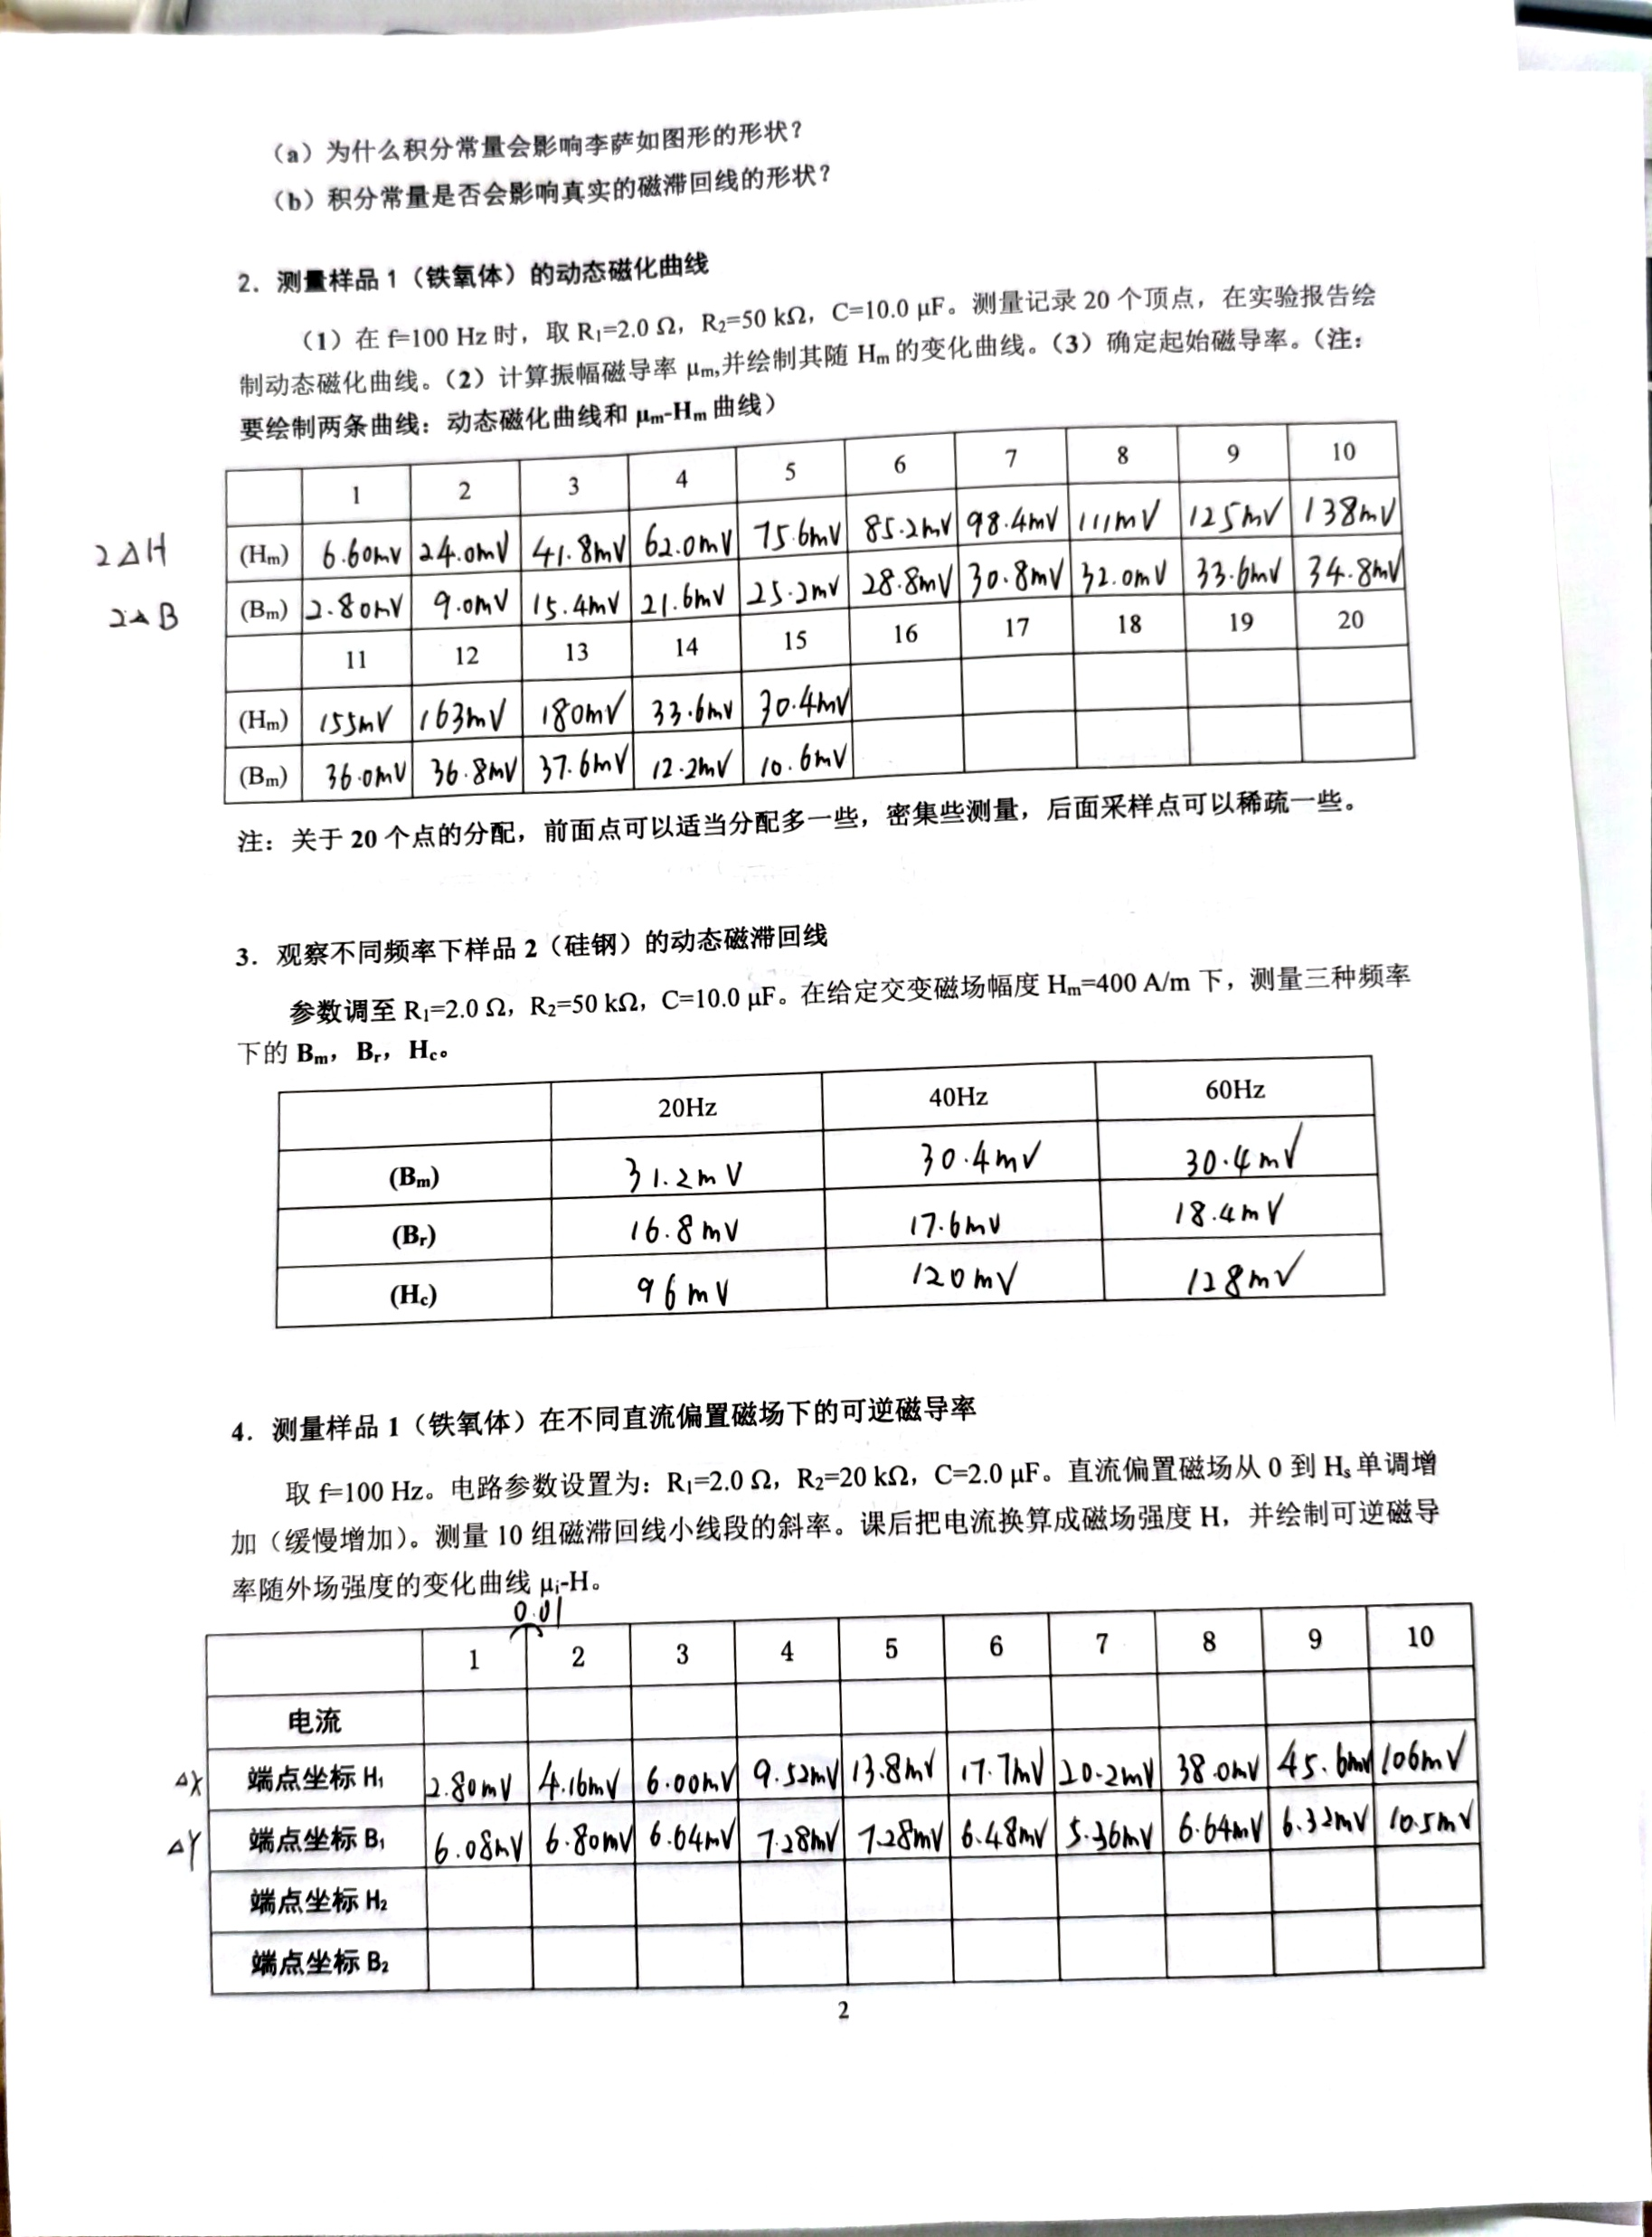
\includegraphics[width=0.9\textwidth]{IMG_20260204_184332.jpg}
    \caption{实验记录2}
\end{figure}
\begin{figure}
    \centering
    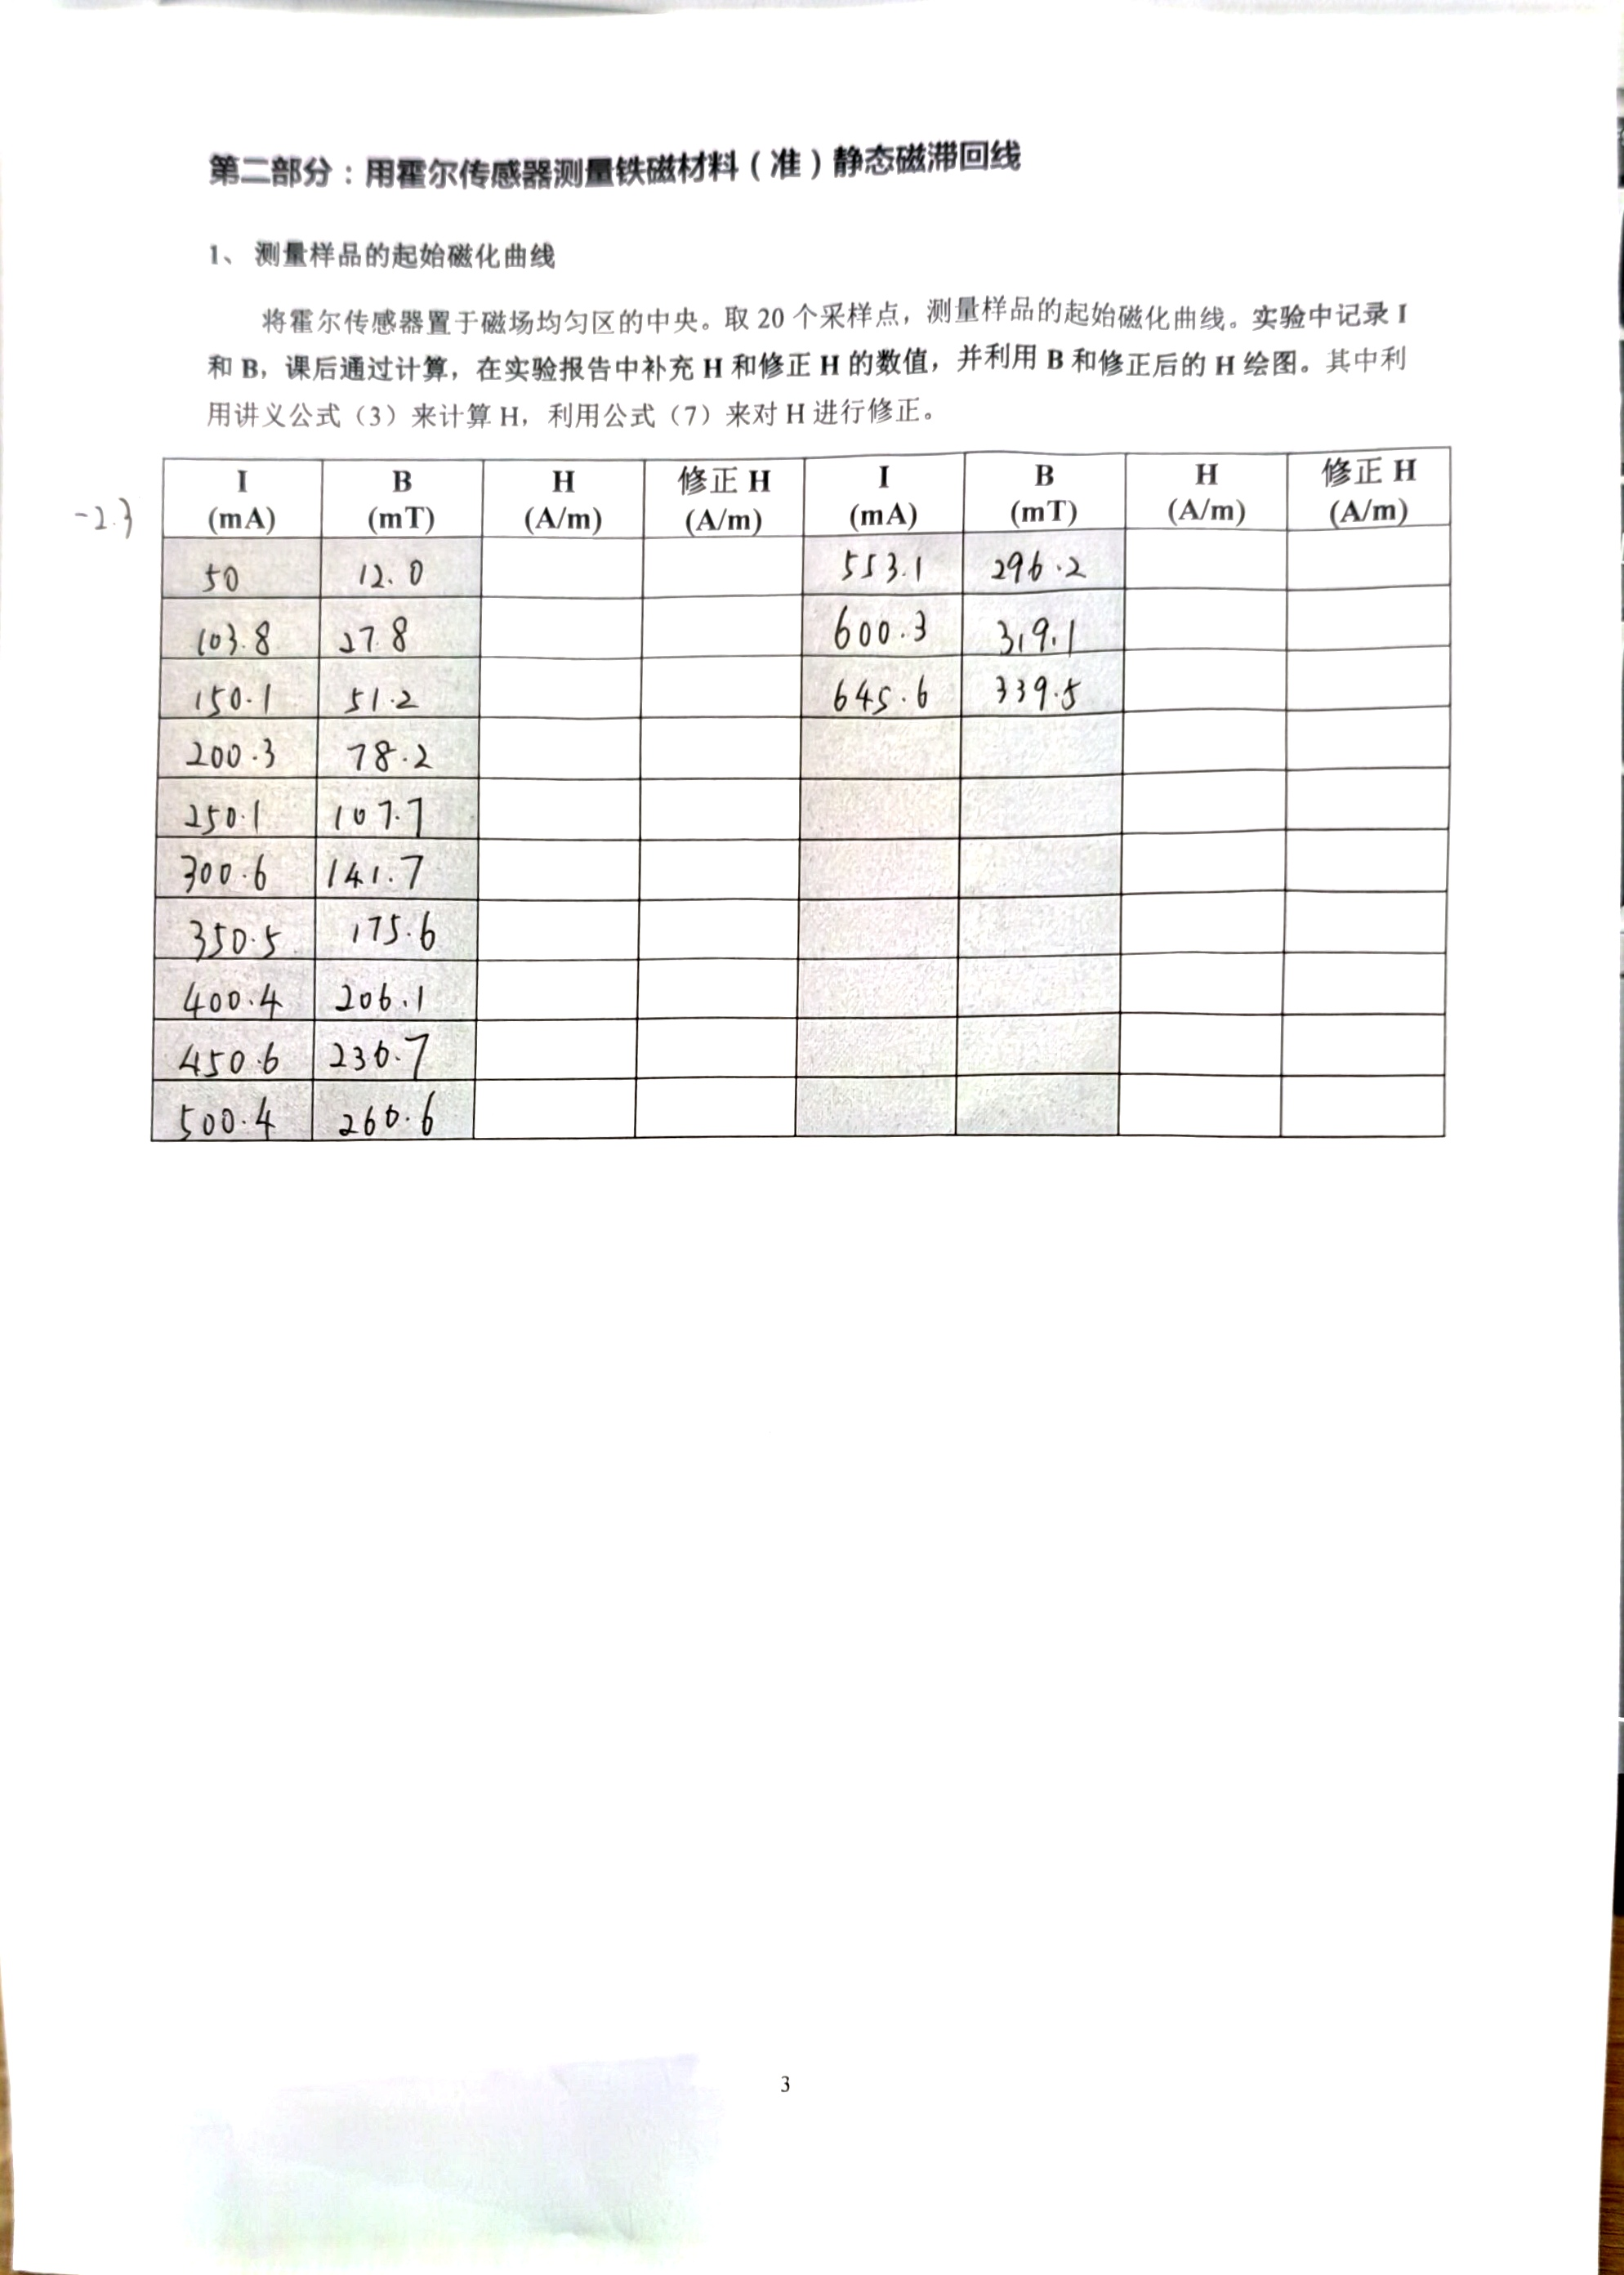
\includegraphics[width=0.9\textwidth]{IMG_20260204_184339.jpg}
    \caption{实验记录3}
\end{figure}
\begin{figure}
    \centering
    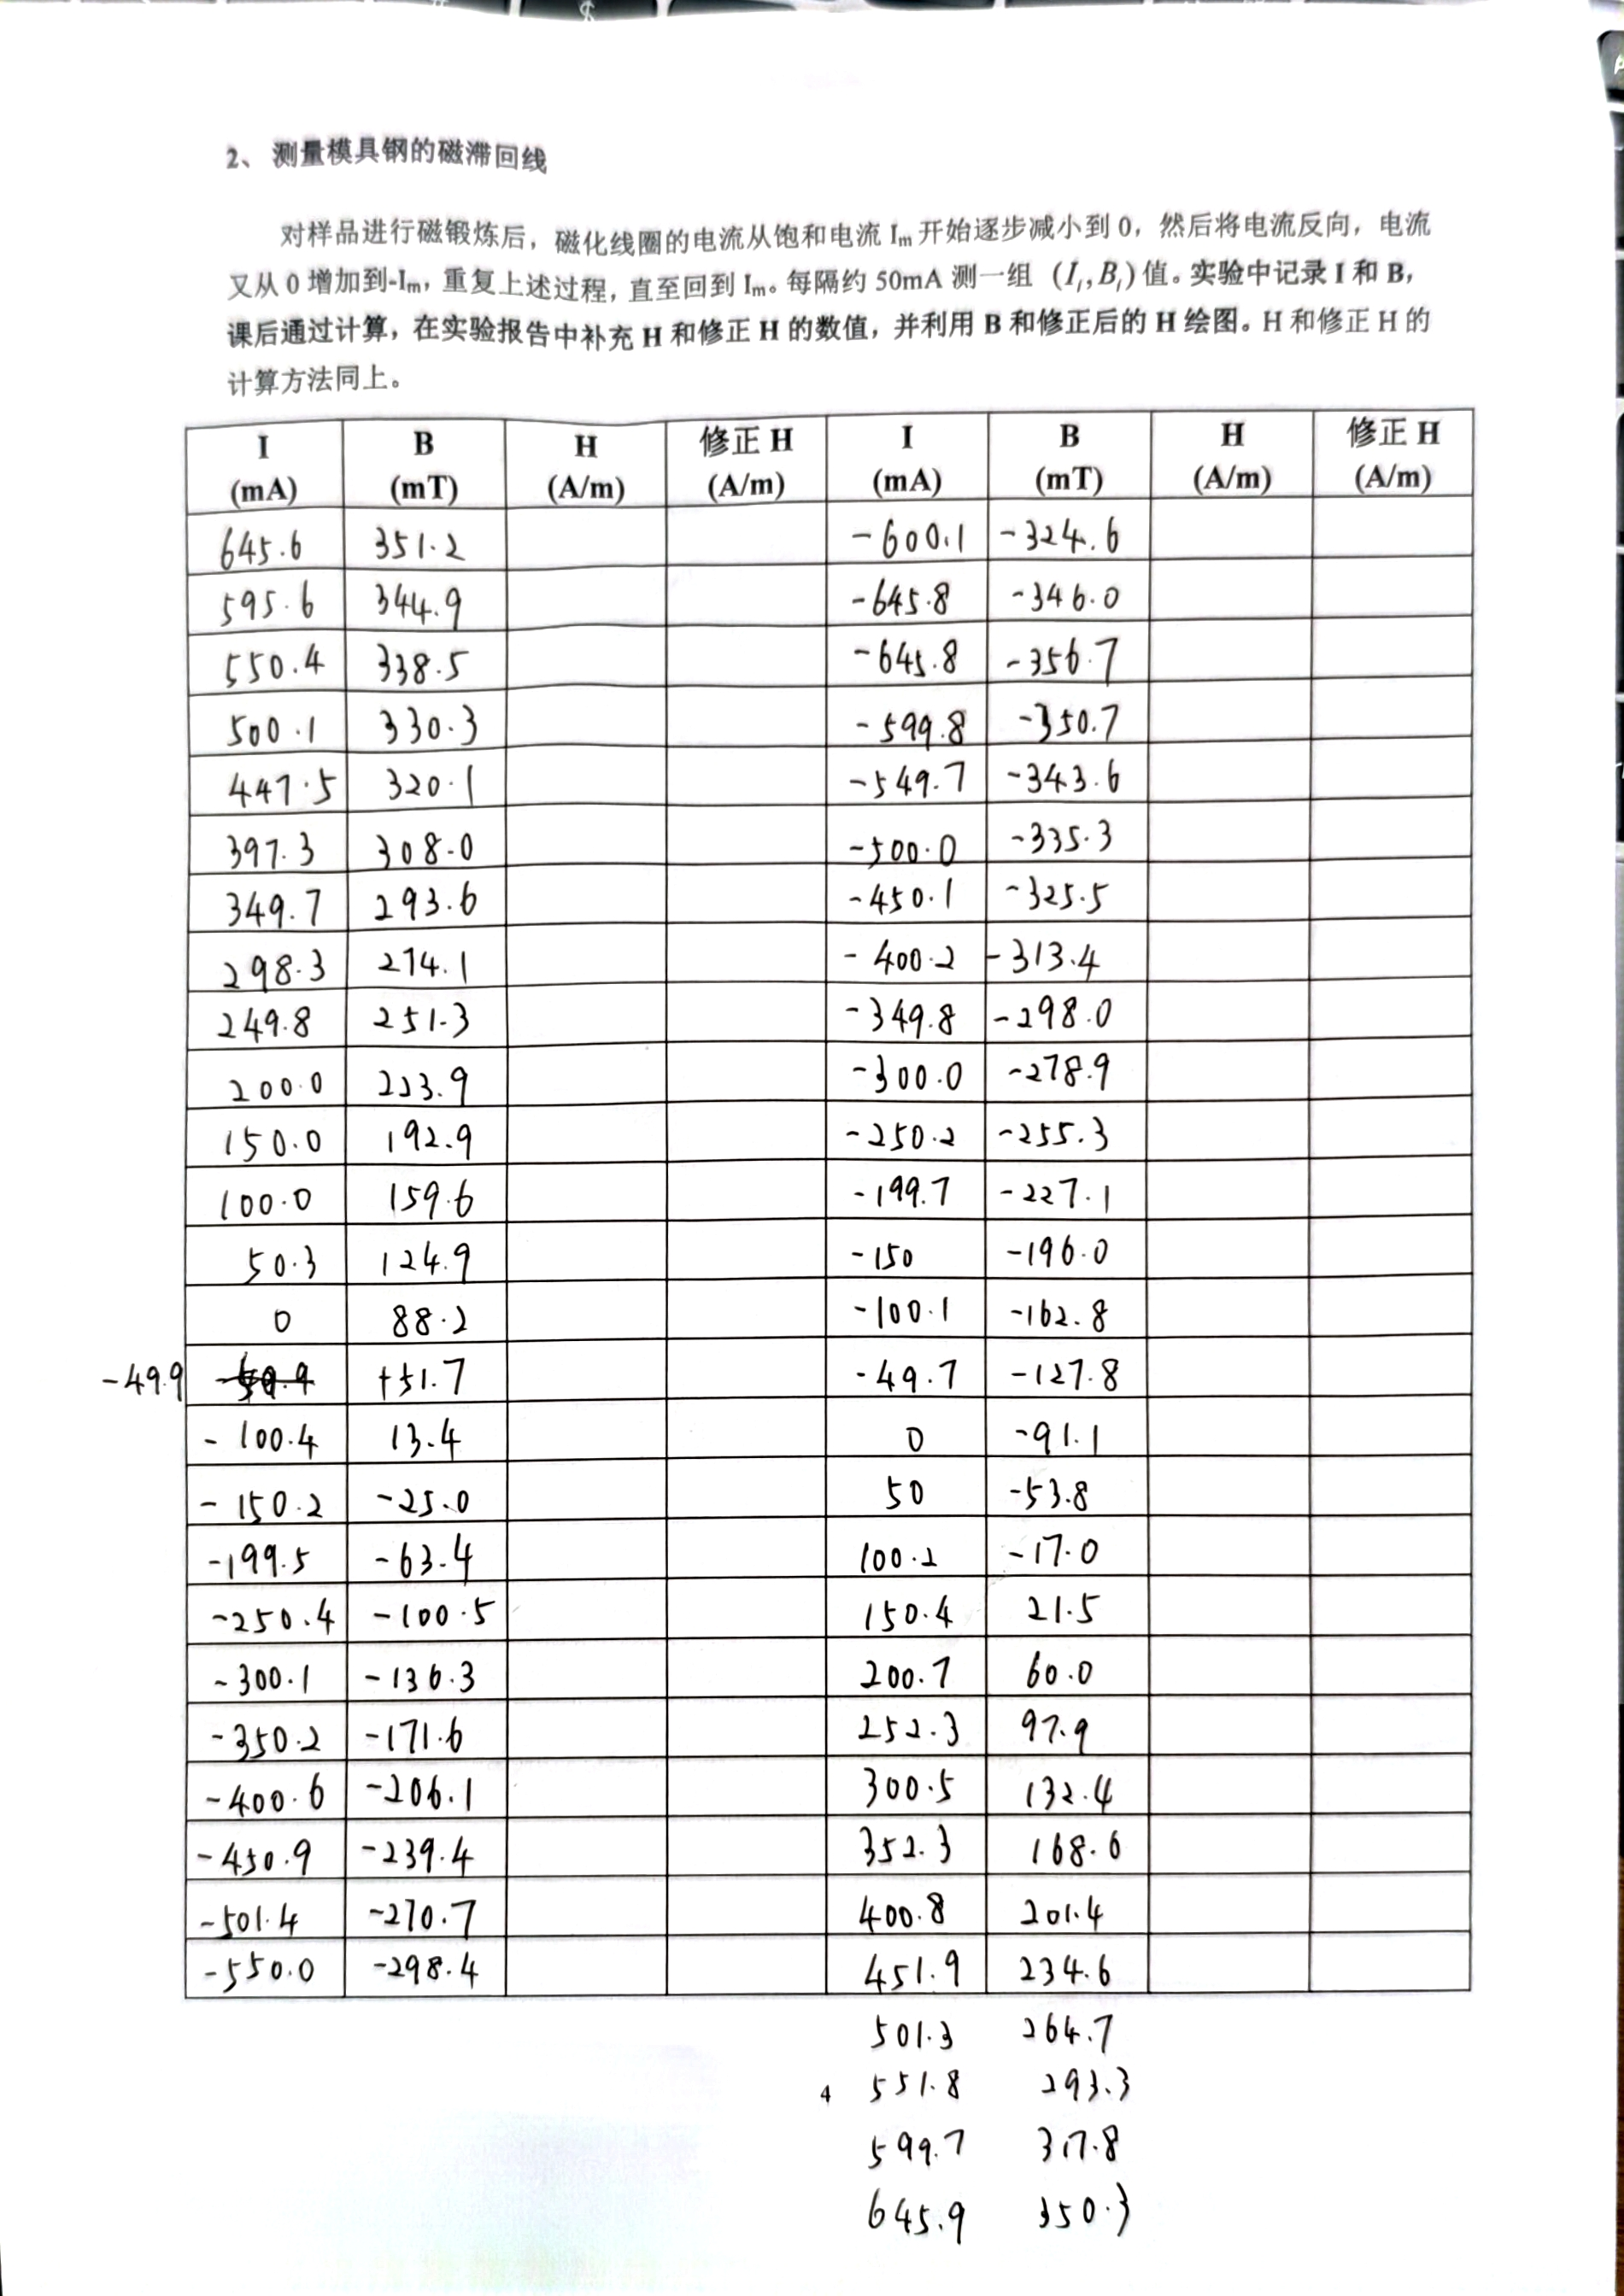
\includegraphics[width=0.9\textwidth]{IMG_20260204_184505.jpg}
    \caption{实验记录4}
\end{figure}
\end{document}